\chapter{运算与周期}
\label{chap:period_foundation}

\markboth{周期基础}{周期基础}

\begin{remark}[本章定位与两条逻辑链]\label{rem:chapter_positioning}
周期性的根源是变换下的不变性。本章以迭代为一切概念的出发点，逐一审查每个箭头的真实逻辑方向与成立条件。核心结论是：在本章的纯代数框架下，\textbf{有限阶作用是得到一致周期与闭合轨道的直接充分必要条件}；守恒与对称是\textbf{发现}有限阶的辅助工具，而非周期存在的必要环节。

因此本章区分两条链：

\[
\boxed{\text{核心判据链：有限阶作用}\Longrightarrow\text{闭合轨道}\Longrightarrow\text{周期}}
\]

\[
\boxed{\text{辅助发现链：守恒}\longleftarrow\text{对称}\quad\text{（用于发现有限阶）}}
\]

核心判据链在双射框架下是充分必要的；辅助发现链是启发式的，方向常常是反的。具体地：
\begin{itemize}
    \item 对称 $\Rightarrow$ 守恒（有条件），而非守恒 $\Rightarrow$ 对称；
    \item 周期 $\Rightarrow$ 对称（演化群自身即有限循环群），但周期 $\nRightarrow$ 非平凡守恒；
    \item 对称与守恒的合取仍 $\nRightarrow$ 周期。
\end{itemize}

本章主要使用集合论、群论与群表示论的代数语言；涉及拓扑的概念仅作启发性说明。
\end{remark}

\section{群论基础与群作用}
\label{sec:group_theory}

本节自洽地建立本章所需的群论语言：群、子群、同态、商群、元素的阶、循环群、群作用、轨道与稳定化子。记号在本节固定，全章通用。

\subsection{群、子群与同态}

\begin{definition}[群]\label{def:group}
一个\textbf{群}是有序对 $(G,\cdot)$，其中 $G$ 为非空集合，$\cdot:G\times G\to G$ 为二元运算，满足：
\begin{enumerate}[label=(\arabic*)]
    \item \textbf{封闭性}：对任意 $a,b\in G$，$a\cdot b\in G$；
    \item \textbf{结合律}：对任意 $a,b,c\in G$，$(a\cdot b)\cdot c=a\cdot(b\cdot c)$；
    \item \textbf{单位元}：存在 $e\in G$，使对任意 $a\in G$，$e\cdot a=a\cdot e=a$；
    \item \textbf{逆元}：对任意 $a\in G$，存在 $a^{-1}\in G$，使 $a\cdot a^{-1}=a^{-1}\cdot a=e$。
\end{enumerate}
\end{definition}

\begin{definition}[阿贝尔群]\label{def:abelian_group}
群 $(G,\cdot)$ 称为\textbf{阿贝尔群}（或交换群），若对任意 $a,b\in G$，
\[
a\cdot b=b\cdot a.
\]
阿贝尔群的运算常记为加法 $+$，单位元记为 $0$，逆元记为 $-a$；此时幂规则写为倍数规则 $n(a+b)=na+nb$。
\end{definition}

\begin{example}[三个基本阿贝尔群]\label{ex:three_abelian_groups}
以下三个阿贝尔群是本章变换理论的代数载体：
\begin{enumerate}[label=(\roman*)]
    \item \textbf{整数加法群} $(\mathbb{Z},+)$：单位元 $0$，$a$ 的逆元 $-a$。这是离散平移的代数基础。
    \item \textbf{正实数乘法群} $(\mathbb{R}^+,\times)$：单位元 $1$，$a$ 的逆元 $1/a$。这是缩放的代数基础。
    \item \textbf{圆群} $U(1)=\{z\in\mathbb{C}\mid |z|=1\}$（复数乘法）：单位元 $1$，$z$ 的逆元 $\bar z$。其运算是复数幂的乘法
    \[
    e^{i\theta}\cdot e^{i\phi}=e^{i(\theta+\phi)}.
    \]
    这是旋转的代数基础。
\end{enumerate}
三者都是阿贝尔群；但它们的\textbf{扭结构}截然不同，这一差异将在定理 \ref{thm:order_structure} 中成为周期理论的焦点。
\end{example}

\begin{definition}[子群]\label{def:subgroup}
设 $G$ 为群，$H\subseteq G$ 非空。若 $H$ 在 $G$ 的运算下自身构成群，则称 $H$ 为 $G$ 的\textbf{子群}，记 $H\le G$。
\end{definition}

\begin{proposition}[子群判据]\label{prop:subgroup_criterion}
设 $G$ 为群，$H\subseteq G$ 非空。则 $H\le G$ 当且仅当：
\begin{enumerate}[label=(\roman*)]
    \item 对任意 $a,b\in H$，$ab\in H$；
    \item 对任意 $a\in H$，$a^{-1}\in H$。
\end{enumerate}
等价地，$H\le G$ 当且仅当对任意 $a,b\in H$，$ab^{-1}\in H$。
\end{proposition}

\begin{proof}
必要性：若 $H$ 为子群，则封闭性 (i) 与逆元封闭 (ii) 由子群定义直接得到。充分性：由 (i) 得封闭性，结合律继承自 $G$。由 (ii) 与 (i)，取 $a\in H$，则 $aa^{-1}=e\in H$，故单位元存在；逆元由 (ii) 给出。等价判据由 $b^{-1}\in H$ 与 $ab^{-1}\in H$ 直接推出。
\end{proof}

\begin{definition}[群同态与同构]\label{def:homomorphism}
设 $G,H$ 为群。映射 $\varphi:G\to H$ 称为\textbf{群同态}，若
\[
\varphi(ab)=\varphi(a)\varphi(b),\qquad \forall a,b\in G.
\]
若 $\varphi$ 为双射，则称为\textbf{群同构}，记 $G\cong H$。同态 $\varphi$ 的\textbf{核}与\textbf{像}分别为
\[
\ker\varphi=\{g\in G\mid \varphi(g)=e_H\},\qquad
\operatorname{im}\varphi=\{\varphi(g)\mid g\in G\}.
\]
\end{definition}

\begin{definition}[正规子群与商群]\label{def:normal_subgroup}
设 $N\le G$。若对任意 $g\in G$，$gN=Ng$，则称 $N$ 为 $G$ 的\textbf{正规子群}，记 $N\trianglelefteq G$。此时陪集集合
\[
G/N=\{gN\mid g\in G\}
\]
在运算 $(gN)(hN)=(gh)N$ 下构成群，称为\textbf{商群}。
\end{definition}

\begin{theorem}[同态基本定理]\label{thm:first_isomorphism}
设 $\varphi:G\to H$ 为群同态。则
\[
G/\ker\varphi\cong \operatorname{im}\varphi.
\]
特别地，$\ker\varphi\trianglelefteq G$。
\end{theorem}

\begin{proof}
令 $K=\ker\varphi$。对任意 $g\in G$，定义 $\bar\varphi(gK)=\varphi(g)$。若 $gK=hK$，则 $h^{-1}g\in K$，故 $\varphi(h^{-1}g)=e$，从而 $\varphi(g)=\varphi(h)$，映射良定义。同态性由 $\varphi$ 的同态性直接得到。核为 $K$，故单射；像为 $\operatorname{im}\varphi$，故满射到像上。于是 $G/K\cong \operatorname{im}\varphi$。
\end{proof}

\begin{figure}[htbp]
\centering
\begin{tikzpicture}[>=stealth, node distance=2.8cm]
    \node (G) {$G$};
    \node[right=of G] (H) {$H$};
    \node[below=of G] (Q) {$G/\ker\varphi$};
    \node[below=of H] (I) {$\operatorname{im}\varphi$};

    \draw[->, thick] (G) -- node[above] {$\varphi$} (H);
    \draw[->, thick] (G) -- node[left] {$\pi$} (Q);
    \draw[->, thick] (Q) -- node[below] {$\cong$} (I);
    \draw[->, thick] (I) -- node[right] {$\iota$} (H);

    \node[font=\footnotesize, below=0.7cm of Q, align=center]
        {$\pi$：自然投影\\ $\iota$：包含映射};
\end{tikzpicture}
\caption{同态基本定理：$G/\ker\varphi\cong\operatorname{im}\varphi$。任意同态 $\varphi$ 都可分解为“投影—同构—包含”。}
\label{fig:first_isomorphism}
\end{figure}

\begin{definition}[中心化子]\label{def:centraliser}
设 $G$ 为群，$S\subseteq G$。$S$ 在 $G$ 中的\textbf{中心化子}为
\[
C_G(S)=\{g\in G\mid gs=sg,\ \forall s\in S\}.
\]
$G$ 的\textbf{中心}为 $Z(G)=C_G(G)$。
\end{definition}

\begin{proposition}[中心化子是子群]\label{prop:centraliser_subgroup}
对任意 $S\subseteq G$，有 $C_G(S)\le G$，且 $Z(G)\trianglelefteq G$。
\end{proposition}

\begin{proof}
$e\in C_G(S)$。若 $a,b\in C_G(S)$，则对任意 $s\in S$，
\[
(ab)s=a(bs)=a(sb)=(as)b=(sa)b=s(ab),
\]
故 $ab\in C_G(S)$。又 $as=sa$ 蕴含 $a^{-1}s=sa^{-1}$，故 $a^{-1}\in C_G(S)$。由子群判据得 $C_G(S)\le G$。中心同理。
\end{proof}

\begin{property}[阿贝尔群的幂规则]\label{prop:abelian_power}
设 $G$ 为阿贝尔群，$a,b\in G$，$n\in\mathbb{Z}$。则
\[
(ab)^n=a^n b^n.
\]
\end{property}

\begin{proof}
先设 $n\ge 0$，对 $n$ 归纳。$n=0$：$(ab)^0=e=ee=a^0b^0$。设 $(ab)^n=a^n b^n$，则
\[
(ab)^{n+1}=(ab)^n(ab)=a^n b^n a b=a^n a b^n b=a^{n+1}b^{n+1},
\]
其中第三步用了交换律 $b^n a=a b^n$。$n<0$ 时，
\[
(ab)^n=((ab)^{-1})^{-n}=(a^{-1}b^{-1})^{-n}=(a^{-1})^{-n}(b^{-1})^{-n}=a^n b^n.
\]
\end{proof}

\begin{remark}[交换律的必要性]\label{rem:abelian_power_necessary}
幂规则 $(ab)^n=a^n b^n$ 在非阿贝尔群中一般不成立：$(ab)^2=abab$ 与 $a^2b^2=aabb$ 相等当且仅当 $ba=ab$。交换律正是“两次迭代可以交换次序”的条件。
\end{remark}

\subsection{元素的阶、扭子群与循环群}

\begin{definition}[元素的阶]\label{def:element_order}
设 $g\in G$。若存在最小正整数 $n$ 使 $g^n=e$，则称 $g$ 的\textbf{阶}为 $n$，记 $\operatorname{ord}(g)=n$；否则称 $g$ 的阶为无限，记 $\operatorname{ord}(g)=\infty$。
\end{definition}

\begin{definition}[扭元素与扭子群]\label{def:torsion}
阶有限的元素称为\textbf{扭元素}；所有元素均为扭元素的群称为\textbf{扭群}。群 $G$ 的全体扭元素构成的集合记为
\[
\operatorname{Tor}(G)=\{g\in G\mid \operatorname{ord}(g)<\infty\}.
\]
\end{definition}

\begin{theorem}[阿贝尔群的扭元素构成子群]\label{thm:torsion_subgroup}
设 $G$ 为阿贝尔群。则 $\operatorname{Tor}(G)\le G$，称为 $G$ 的\textbf{扭子群}。
\end{theorem}

\begin{proof}
$e\in\operatorname{Tor}(G)$。设 $a,b\in\operatorname{Tor}(G)$，$\operatorname{ord}(a)=m$，$\operatorname{ord}(b)=n$。由性质 \ref{prop:abelian_power}，
\[
(ab)^{mn}=a^{mn}b^{mn}=(a^m)^n(b^n)^m=e.
\]
故 $\operatorname{ord}(ab)\le mn<\infty$，$ab\in\operatorname{Tor}(G)$。又 $(a^{-1})^m=(a^m)^{-1}=e$，故 $a^{-1}\in\operatorname{Tor}(G)$。由子群判据，$\operatorname{Tor}(G)\le G$。
\end{proof}

\begin{remark}[非阿贝尔群中扭元素不封闭]\label{rem:torsion_nonabelian}
定理 \ref{thm:torsion_subgroup} 的证明本质地使用交换律，且结论在非阿贝尔群中确实失效。例如在 $\mathrm{GL}_2(\mathbb{R})$ 中取
\[
A=\begin{pmatrix}0&1\\1&0\end{pmatrix},\qquad
B=\begin{pmatrix}0&2\\1/2&0\end{pmatrix},
\]
则 $A^2=B^2=I$，但 $AB=\operatorname{diag}(1/2,2)$，$(AB)^n=\operatorname{diag}(2^{-n},2^n)\neq I$ 对一切 $n\ge 1$ 成立，故 $\operatorname{ord}(AB)=\infty$。
\end{remark}

\begin{definition}[陪集与指数]\label{def:coset_index}
设 $H\le G$。对 $g\in G$，左陪集与右陪集分别为
\[
gH=\{gh\mid h\in H\},\qquad Hg=\{hg\mid h\in H\}.
\]
若 $G$ 有限，$H$ 在 $G$ 中的\textbf{指数}为左陪集的个数，记
\[
[G:H]=\frac{|G|}{|H|}.
\]
\end{definition}

\begin{lemma}[拉格朗日]\label{lem:lagrange}
设 $G$ 为有限群，$H\le G$。则 $|H|\mid |G|$，且 $|G|=[G:H]|H|$。
\end{lemma}

\begin{proof}
左陪集族 $\{gH\mid g\in G\}$ 构成 $G$ 的划分：$g\in gH$ 给出覆盖；若 $gH\cap g'H\neq\emptyset$，设 $gh=g'h'$，则 $g'=gh(h')^{-1}\in gH$，从而 $g'H\subseteq gH$，对称地 $gH\subseteq g'H$，故陪集或相等或不交。每个陪集与 $H$ 等势：$h\mapsto gh$ 是 $H\to gH$ 的双射。设陪集个数为 $[G:H]$，则 $|G|=[G:H]|H|$。
\end{proof}

\begin{proposition}[有限群中元素的阶]\label{prop:order_divides}
设 $G$ 为有限群，$g\in G$。则 $\operatorname{ord}(g)<\infty$ 且 $\operatorname{ord}(g)\mid |G|$。
\end{proposition}

\begin{proof}
序列 $g,g^2,g^3,\dots$ 取值于有限集 $G$，必存在 $i<j$ 使 $g^i=g^j$，于是 $g^{j-i}=e$，阶有限。设 $n=\operatorname{ord}(g)$，则 $\langle g\rangle=\{e,g,\dots,g^{n-1}\}$ 恰含 $n$ 个元素，即 $|\langle g\rangle|=n$。由引理 \ref{lem:lagrange}，$n\mid |G|$。
\end{proof}

\begin{corollary}[素数阶群是循环群]\label{cor:prime_order}
设 $|G|=p$ 为素数。则 $G$ 是循环群，且任意 $g\neq e$ 都是生成元。
\end{corollary}

\begin{proof}
取 $g\neq e$。由命题 \ref{prop:order_divides}，$\operatorname{ord}(g)\mid p$ 且 $\operatorname{ord}(g)\ge 2$，故 $\operatorname{ord}(g)=p$，$\langle g\rangle=G$。
\end{proof}

\begin{definition}[循环群]\label{def:cyclic_group}
群 $G$ 称为\textbf{循环群}，若存在 $g\in G$ 使
\[
G=\langle g\rangle=\{g^n\mid n\in\mathbb{Z}\}.
\]
$g$ 称为 $G$ 的\textbf{生成元}。
\end{definition}

\begin{proposition}[循环群是阿贝尔群]\label{prop:cyclic_abelian}
循环群必为阿贝尔群。
\end{proposition}

\begin{proof}
设 $G=\langle g\rangle$。任取 $a,b\in G$，则 $a=g^m$，$b=g^n$，于是
\[
ab=g^m g^n=g^{m+n}=g^{n+m}=g^n g^m=ba.
\]
\end{proof}

\begin{proposition}[循环群的分类]\label{prop:cyclic_classification}
设 $G=\langle g\rangle$ 为循环群。则：
\begin{enumerate}[label=(\roman*)]
    \item 若 $\operatorname{ord}(g)=\infty$，则 $G\cong(\mathbb{Z},+)$；
    \item 若 $\operatorname{ord}(g)=n<\infty$，则 $G\cong(\mathbb{Z}/n\mathbb{Z},+)$。
\end{enumerate}
\end{proposition}

\begin{proof}
(i) 映射 $\varphi:\mathbb{Z}\to G$，$\varphi(k)=g^k$ 是满同态；若 $\varphi(k)=\varphi(l)$，则 $g^{k-l}=e$，由阶无限得 $k=l$，故 $\varphi$ 单射，从而是同构。

(ii) 映射 $\varphi:\mathbb{Z}/n\mathbb{Z}\to G$，$\varphi([k])=g^k$ 良定义；满射：对任意 $g^k\in G$，取 $[k]$ 即有原像；若 $g^k=g^l$，则 $g^{k-l}=e$，由阶的定义 $n\mid(k-l)$，即 $[k]=[l]$，单射。故为同构。
\end{proof}

\begin{lemma}[有限循环群中元素的阶]\label{lem:order_cyclic}
设 $m\ge 1$。在加法群 $\mathbb{Z}/m\mathbb{Z}$ 中，元素 $[T]$ 的阶为
\[
\operatorname{ord}([T])=\frac{m}{\gcd(T,m)}.
\]
特别地，$[T]$ 生成整个 $\mathbb{Z}/m\mathbb{Z}$ 当且仅当 $\gcd(T,m)=1$。
\end{lemma}

\begin{proof}
$[T]$ 的阶是使 $nT\equiv 0\pmod m$ 成立的最小正整数 $n$。设 $d=\gcd(T,m)$，则
\[
m\mid nT \iff \frac{m}{d}\mid n\cdot\frac{T}{d}.
\]
因 $\gcd(m/d,T/d)=1$，得 $m/d\mid n$，最小正整数解为 $n=m/d$。当 $d=1$ 时阶为 $m$，故 $[T]$ 为生成元；反之若 $[T]$ 生成全群，则其阶为 $m$，即 $m=m/d$，得 $d=1$。
\end{proof}

\begin{figure}[htbp]
\centering
\begin{tikzpicture}[scale=1.0,>=stealth]
    \draw[thick, gray] (0,0) circle (1.8);
    \foreach \k in {0,1,...,11} {
        \filldraw[blue!70!black] ({\k*30}:1.8) circle (2.2pt);
    }

    \foreach \k/\lab in {0/0, 3/3, 6/6, 9/9} {
        \node[font=\footnotesize, blue!70!black] at ({\k*30}:2.1) {$\lab$};
    }

    \draw[->, thick, red!70!black] (30:1.8) arc (30:60:1.8);
    \draw[->, thick, red!70!black] (60:1.8) arc (60:90:1.8);
    \node[red!70!black, font=\footnotesize] at (1.2,1.4) {$+1$};

    \node[font=\small\bfseries, below=2.5cm] at (0,0)
        {$\operatorname{ord}([T])=\dfrac{m}{\gcd(T,m)}$};
\end{tikzpicture}
\caption{循环群 $\mathbb Z/m\mathbb Z$ 上的平移 $x\mapsto x+1$。步长 $T$ 的实际周期由 $\gcd(T,m)$ 决定：$[T]$ 生成全群当且仅当 $\gcd(T,m)=1$。}
\label{fig:cyclic_order}
\end{figure}

\begin{remark}[循环群：周期的代数原型]\label{rem:cyclic_prototype}
循环群是本章最重要的对象：闭合轨道上的动力学同构于循环群的平移；周期系统自带的演化群也是循环群。引理 \ref{lem:order_cyclic} 表明：循环群内部还存在\textbf{子周期}的丰富层次——步长 $T$ 与模 $m$ 的最大公因数决定实际周期。
\end{remark}

\subsection{群作用、轨道与稳定化子}

\begin{definition}[群作用、轨道与稳定化子]\label{def:group_action}
设 $G$ 为群，$X$ 为集合。$G$ 在 $X$ 上的\textbf{左作用}是映射
\[
\Phi:G\times X\to X,\qquad (g,x)\mapsto g\cdot x,
\]
满足 $e\cdot x=x$ 与 $(gh)\cdot x=g\cdot(h\cdot x)$。点 $x_0\in X$ 的\textbf{轨道}与\textbf{稳定化子}分别为
\[
\mathcal{O}_G(x_0)=\{g\cdot x_0\mid g\in G\},\qquad
\operatorname{Stab}_G(x_0)=\{g\in G\mid g\cdot x_0=x_0\}.
\]
若对任意 $x,y\in X$ 存在 $g\in G$ 使 $y=g\cdot x$，则称作用\textbf{传递}。
\end{definition}

\begin{proposition}[稳定化子是子群]\label{prop:stabilizer_subgroup}
设 $G$ 作用于 $X$，$x_0\in X$。则 $\operatorname{Stab}_G(x_0)\le G$。
\end{proposition}

\begin{proof}
$e\cdot x_0=x_0$，故 $e\in\operatorname{Stab}_G(x_0)$。若 $g,h\in\operatorname{Stab}_G(x_0)$，则
\[
(gh)\cdot x_0=g\cdot(h\cdot x_0)=g\cdot x_0=x_0,
\]
故 $gh\in\operatorname{Stab}_G(x_0)$。又若 $g\cdot x_0=x_0$，则
\[
x_0=e\cdot x_0=(g^{-1}g)\cdot x_0=g^{-1}\cdot(g\cdot x_0)=g^{-1}\cdot x_0,
\]
故 $g^{-1}\in\operatorname{Stab}_G(x_0)$。由子群判据得结论。
\end{proof}

\begin{lemma}[轨道--稳定化子]\label{lem:orbit_stabilizer}
设 $G$ 作用于 $X$，$x_0\in X$。则映射
\[
g\operatorname{Stab}_G(x_0)\mapsto g\cdot x_0
\]
给出双射
\[
G/\operatorname{Stab}_G(x_0)\longleftrightarrow \mathcal{O}_G(x_0),
\]
故
\[
|\mathcal{O}_G(x_0)|=[G:\operatorname{Stab}_G(x_0)].
\]
\end{lemma}

\begin{proof}
记 $H=\operatorname{Stab}_G(x_0)$。若 $gH=hH$，则 $h^{-1}g\in H$，故
\[
g\cdot x_0=h\cdot(h^{-1}g)\cdot x_0=h\cdot x_0,
\]
映射良定义。反之若 $g\cdot x_0=h\cdot x_0$，则 $h^{-1}g\cdot x_0=x_0$，即 $gH=hH$，映射单射。满射：因 $gH=\varphi(g)$，像集即全部陪集。
\end{proof}

\begin{theorem}[轨道划分]\label{thm:orbit_partition}
设 $G$ 作用于 $X$。关系
\[
x\sim y \iff \exists g\in G,\ y=g\cdot x
\]
是 $X$ 上的等价关系，其等价类恰为全体 $G$-轨道。因此全体轨道构成 $X$ 的划分。
\end{theorem}

\begin{proof}
自反性：$x=e\cdot x$。对称性：若 $y=g\cdot x$，则 $x=g^{-1}\cdot y$。传递性：若 $y=g\cdot x$，$z=h\cdot y$，则 $z=(hg)\cdot x$。等价类正是 $\{g\cdot x\mid g\in G\}=\mathcal{O}_G(x)$。
\end{proof}

\begin{remark}[作用的忠实性]\label{rem:faithful}
作用 $\Phi$ 诱导群同态 $\rho:G\to\operatorname{Aut}(X)$，$\rho(g)(x)=g\cdot x$。若 $\rho$ 为单射，称作用是\textbf{忠实}的。本章默认通过 $\rho$ 将 $G$ 视为 $\operatorname{Aut}(X)$ 的子群，从而“元素的阶”与“变换的阶”两个语言系统可以互换使用。
\end{remark}

\begin{figure}[htbp]
\centering
\begin{tikzpicture}[scale=1.0,>=stealth]
    \draw[thick, fill=blue!5] (0,0) ellipse (4 and 2.5);
    \node[font=\small\bfseries, blue!70!black] at (3.2, 2.0) {$X$};

    \draw[thick, red!70!black]
        (0.5,0.3) .. controls (2.5,1.5) and (2.0,-1.5) .. (-0.5,-0.5)
        .. controls (-2.0,0.5) and (-1.5,1.2) .. (0.5,0.3);
    \node[red!70!black, font=\footnotesize] at (2.7, 0.9) {$\mathcal{O}_G(x_0)$};

    \filldraw[black] (0.5, 0.3) circle (2.5pt);
    \node[font=\small, below right=1pt] at (0.5,0.3) {$x_0$};

    \filldraw[black] (-1.5, 0.8) circle (2pt);
    \node[font=\small, above left=1pt] at (-1.5,0.8) {$g\cdot x_0$};

    \draw[thick, fill=green!5] (7,0) ellipse (1.8 and 2.5);
    \node[font=\small\bfseries, green!60!black] at (7, 2.0) {$G$};

    \draw[thick, fill=orange!30] (7,-0.5) ellipse (1.0 and 1.0);
    \node[font=\footnotesize, orange!80!black, align=center] at (7,-0.5)
        {$\operatorname{Stab}_G(x_0)$};

    \draw[->, thick, gray] (5.3, 0.7) to[bend left=20]
        node[above, font=\footnotesize] {作用} (2.5, 1.4);
    \draw[->, thick, gray] (5.3,-1.2) to[bend right=20]
        node[below, font=\footnotesize] {$G/\operatorname{Stab}\cong\mathcal{O}$} (1.2,-1.8);
\end{tikzpicture}
\caption{群作用、轨道与稳定化子。轨道与稳定化子的关系由引理 \ref{lem:orbit_stabilizer} 给出。}
\label{fig:group_action_illustration}
\end{figure}

\section{迭代：一切概念的出发点}

\begin{definition}[迭代与离散动力系统]\label{def:iteration}
设 $X$ 为非空集合，$f:X\to X$ 为映射。定义 $f$ 的\textbf{迭代}为
\[
f^0=\operatorname{id}_X,\qquad f^{n+1}=f\circ f^n\quad(n\ge 0).
\]
有序对 $(X,f)$ 称为一个\textbf{离散动力系统}，$f$ 称为\textbf{生成元}或\textbf{演化映射}。若 $f$ 为双射，定义负次迭代 $f^{-n}=(f^{-1})^n$，从而迭代扩展为整数指标族 $\{f^n\}_{n\in\mathbb{Z}}$。
\end{definition}

\begin{property}[迭代的指数律]\label{prop:iteration_law}
对任意 $m,n\ge 0$（$f$ 双射时 $m,n\in\mathbb{Z}$），
\[
f^{m+n}=f^m\circ f^n,\qquad f^{mn}=(f^m)^n.
\]
特别地，$f$ 双射时映射 $n\mapsto f^n$ 是群同态 $(\mathbb{Z},+)\to\operatorname{Aut}(X)$，即迭代等价于 $\mathbb{Z}$ 在 $X$ 上的作用。
\end{property}

\begin{proof}
对 $n$ 作归纳：$f^{m+0}=f^m=f^m\circ f^0$；设 $f^{m+n}=f^m\circ f^n$，则
\[
f^{m+n+1}=f\circ f^{m+n}=f\circ f^m\circ f^n=f^{m+1}\circ f^n=f^m\circ f^{n+1}.
\]
第二式由第一式对 $n$ 归纳即得。负指标情形由 $(f^{-1})^n$ 的定义与同一归纳推出。同态性正是第一式。
\end{proof}

\begin{remark}[迭代的先在性]\label{rem:iteration_primordial}
迭代在逻辑上先于运算：自然数的加法、乘法、幂本身即由“后继映射的迭代”递归生成。因此本章把迭代而非群运算作为出发点——群只是迭代在可逆情形下自组织出的代数结构。
\end{remark}

\begin{definition}[轨道]\label{def:orbit}
设 $(X,f)$ 为离散动力系统，$x_0\in X$。$x_0$ 的\textbf{前向轨道}为
\[
\mathcal{O}^+(x_0;f)=\{f^n(x_0)\mid n\ge 0\}.
\]
若 $f$ 双射，$x_0$ 的\textbf{（双向）轨道}为
\[
\mathcal{O}(x_0;f)=\{f^n(x_0)\mid n\in\mathbb{Z}\}=\mathcal{O}_{\langle f\rangle}(x_0).
\]
\end{definition}

\begin{proposition}[轨道划分]\label{prop:orbit_partition}
设 $f$ 双射。关系
\[
x\sim y \iff \exists n\in\mathbb{Z},\ y=f^n(x)
\]
是 $X$ 上的等价关系，其等价类恰为全体轨道。因此轨道族构成 $X$ 的划分。
\end{proposition}

\begin{proof}
自反性：$x=f^0(x)$。对称性：$y=f^n(x)\Rightarrow x=f^{-n}(y)$。传递性：$y=f^n(x),z=f^m(y)\Rightarrow z=f^{m+n}(x)$。等价类 $[x]=\{f^n(x)\}=\mathcal{O}(x;f)$。
\end{proof}

\begin{definition}[周期点与最终周期点]\label{def:periodic_point}
设 $(X,f)$ 为离散动力系统，$x_0\in X$。若存在整数 $m\ge 1$ 使
\[
f^m(x_0)=x_0,
\]
则称 $x_0$ 为\textbf{周期点}；满足上式的最小正整数 $m_0$ 称为 $x_0$ 的\textbf{最小周期}。若存在 $k\ge 0$ 使 $f^k(x_0)$ 为周期点，则称 $x_0$ 为\textbf{最终周期点}。
\end{definition}

\begin{example}[最终周期而非周期的点]\label{ex:eventually_periodic}
设 $X=\{0,1,2\}$，$f(0)=1$，$f(1)=2$，$f(2)=1$。则 $f^2(1)=1$，$1$ 与 $2$ 是周期点；$f(0)=1$ 而 $0$ 不在任何回归轨道上，故 $0$ 是最终周期点而非周期点。
\end{example}

\begin{lemma}[可逆演化中的回归]\label{lem:invertible_recurrence}
设 $f$ 双射，$x_0\in X$。若 $x_0$ 为最终周期点，则 $x_0$ 为周期点。
\end{lemma}

\begin{proof}
设 $f^k(x_0)$ 为周期点，$f^m(f^k(x_0))=f^k(x_0)$，$m\ge 1$。两边作用 $f^{-k}$ 得 $f^m(x_0)=x_0$。
\end{proof}

\begin{figure}[htbp]
\centering
\begin{tikzpicture}[scale=0.95,>=stealth]

    \begin{scope}[shift={(-4.2,0)}]
        \draw[gray!40] (0,0) circle (1.4);
        \foreach \k in {0,1,...,5} {
            \filldraw[blue!70!black] ({60*\k}:1.4) circle (2.2pt);
        }
        \foreach \k in {0,1,...,5} {
            \draw[->, thick, blue!70!black] ({60*\k}:1.4) arc ({60*\k}:{60*(\k+1)}:1.4);
        }
        \node[font=\small\bfseries, below=2.0cm] at (0,0)
            {(a) 周期点：$f^m(x_0)=x_0$};
    \end{scope}

    \begin{scope}[shift={(0,0)}]
        \draw[gray!40] (0,0) circle (1.4);
        \foreach \k in {0,1,...,3} {
            \filldraw[blue!70!black] ({90*\k}:1.4) circle (2.2pt);
        }
        \draw[->, thick, red!70!black]
            (-2.5,1.4) .. controls (-1.6,1.9) and (-0.8,1.7) .. (-0.3,1.5)
            .. controls (0.0,1.6) and (0.2,1.5) .. (0,1.4);
        \node[red!70!black, font=\footnotesize] at (-2.0,2.0) {$x_0$};
        \foreach \k in {0,1,...,3} {
            \draw[->, thick, blue!70!black] ({90*\k}:1.4) arc ({90*\k}:{90*(\k+1)}:1.4);
        }
        \node[font=\small\bfseries, below=2.0cm] at (0,0)
            {(b) 最终周期：先进入循环};
    \end{scope}

    \begin{scope}[shift={(4.2,0)}]
        \draw[gray!40, fill=blue!3] (0,0) ellipse (1.6 and 1.4);
        \draw[thick, red!70!black]
            (0,0) .. controls (0.3,0.2) and (0.6,0.5) .. (0.4,0.8)
            .. controls (0.1,1.1) and (-0.5,1.1) .. (-0.9,0.7)
            .. controls (-1.3,0.3) and (-1.2,-0.4) .. (-0.7,-0.9)
            .. controls (-0.1,-1.4) and (0.8,-1.3) .. (1.2,-0.7)
            .. controls (1.6,-0.1) and (1.5,0.8) .. (0.9,1.3);
        \filldraw[red!70!black] (0,0) circle (2.2pt);
        \node[red!70!black, font=\footnotesize] at (0.4,-0.4) {$x_0$};
        \node[font=\small\bfseries, below=2.0cm] at (0,0)
            {(c) 非周期：轨道无限不闭合};
    \end{scope}

\end{tikzpicture}
\caption{三类轨道的几何形态：周期轨道闭合；最终周期轨道先经有限步后进入闭合循环；非周期轨道无限延伸而不闭合。}
\label{fig:iteration_orbit_types}
\end{figure}

\section{不变量与守恒}
\label{sec:invariants_conservation}

\begin{definition}[不变量（守恒量）]\label{def:invariant}
设 $(X,f)$ 为离散动力系统。映射 $Q:X\to Y$ 称为 $f$ 的\textbf{不变量}，若
\[
Q\circ f=Q,\qquad\text{即}\qquad Q(f(x))=Q(x),\quad\forall x\in X.
\]
当 $Y=\mathbb{R}$ 时，$Q$ 又称为\textbf{守恒量}或\textbf{首积分}。若 $Q$ 为常值映射，称其为\textbf{平凡不变量}；否则为\textbf{非平凡不变量}。
\end{definition}

\begin{proposition}[不变量的轨道刻划]\label{prop:invariant_orbit}
$Q$ 是 $f$ 的不变量，当且仅当 $Q$ 在每条前向轨道上取常值；当 $f$ 双射时，当且仅当 $Q$ 在每条双向轨道上取常值。
\end{proposition}

\begin{proof}
若 $Q\circ f=Q$，则对 $n$ 归纳得 $Q\circ f^n=Q$，故 $Q$ 在 $\{f^n(x_0)\}$ 上恒为 $Q(x_0)$。反之，若 $Q$ 在每条前向轨道上恒定，则对任意 $x$，$Q(f(x))=Q(x)$。双射情形同理。
\end{proof}

\begin{property}[不变量的代数封闭性]\label{prop:invariant_algebra}
设 $Q_1,Q_2:X\to\mathbb{R}$ 为 $f$-守恒量，$\varphi:\mathbb{R}^2\to\mathbb{R}$ 为任意映射。则 $x\mapsto\varphi(Q_1(x),Q_2(x))$ 仍为 $f$-守恒量。特别地，$f$-守恒量的全体构成 $\mathbb{R}$-代数。
\end{property}

\begin{proof}
逐点验证：
\[
\varphi(Q_1(f(x)),Q_2(f(x)))=\varphi(Q_1(x),Q_2(x)).
\]
\end{proof}

\begin{remark}[平凡性：存在守恒量不是条件]\label{rem:trivial_invariant}
常值映射总是 $f$ 的不变量，故“存在守恒量”对任何系统成立，不构成任何约束。有判别力的陈述是“存在\textbf{非平凡}守恒量”。因此把“存在守恒量”列为周期的必要条件是疏漏：若“守恒”含平凡情形则该条件恒真、无信息量；若要求非平凡，则周期系统也未必满足。
\end{remark}

\begin{definition}[守恒群]\label{def:conservation_group}
设 $Q:X\to Y$。$Q$ 的\textbf{守恒群}（等变群）为
\[
G_Q=\{g\in\operatorname{Aut}(X)\mid Q\circ g=Q\}.
\]
\end{definition}

\begin{property}[守恒群是群]\label{prop:conservation_group_is_group}
$G_Q\le\operatorname{Aut}(X)$。
\end{property}

\begin{proof}
$\operatorname{id}_X\in G_Q$。若 $Q\circ g=Q$ 且 $Q\circ h=Q$，则 $Q\circ(g\circ h)=Q$，且
\[
Q\circ g^{-1}=(Q\circ g)\circ g^{-1}=Q.
\]
故 $G_Q$ 对复合与取逆封闭。
\end{proof}

\begin{proposition}[演化守恒其自身的不变量]\label{prop:f_in_GQ}
设 $f$ 双射且 $Q$ 为 $f$-不变量。则 $\langle f\rangle\le G_Q$。
\end{proposition}

\begin{proof}
由命题 \ref{prop:invariant_orbit}，$Q\circ f^n=Q$ 对所有 $n\in\mathbb{Z}$ 成立。故 $f^n\in G_Q$。
\end{proof}

\begin{remark}[守恒量的三种来源]\label{rem:conservation_source}
守恒量的识别有三条途径：\textbf{经验观察}；\textbf{对称性推导}；\textbf{数学结构}（轨道等价类的标签函数）。三者都产生轨道常值函数。
\end{remark}

\begin{figure}[htbp]
\centering
\begin{tikzpicture}[scale=1.0,>=stealth]
    \draw[->, gray] (-0.5,0) -- (5.5,0) node[right, font=\scriptsize] {$x$};
    \draw[->, gray] (0,-0.5) -- (0,4.2) node[above, font=\scriptsize] {$Q$};

    \draw[thick, blue!70!black, domain=0.2:5.2, samples=120]
        plot (\x, {1.0+0.7*sin(120*\x)});
    \draw[thick, red!70!black, domain=0.2:5.2, samples=120]
        plot (\x, {2.3+0.7*sin(120*\x+60)});
    \draw[thick, green!60!black, domain=0.2:5.2, samples=120]
        plot (\x, {3.6+0.7*sin(120*\x+120)});

    \node[blue!70!black, font=\footnotesize] at (5.0,1.2) {$Q=c_1$};
    \node[red!70!black, font=\footnotesize] at (5.0,2.5) {$Q=c_2$};
    \node[green!60!black, font=\footnotesize] at (5.0,3.8) {$Q=c_3$};

    \draw[->, thick, orange!80!black] (0.8,1.0) -- (1.6,1.0);
    \draw[->, thick, orange!80!black] (1.6,1.0) -- (2.4,1.0);
    \node[orange!80!black, font=\footnotesize] at (1.6,0.6) {轨道};
\end{tikzpicture}
\caption{守恒量 $Q$ 的几何图像：$Q$ 在每条轨道上取常值，因此轨道被限制在 $Q$ 的水平集内。不同水平集给出轨道之间的分层。}
\label{fig:invariant_level_sets}
\end{figure}

\section{对称}

\begin{definition}[动力系统的对称群]\label{def:symmetry_group}
设 $(X,f)$ 为离散动力系统，$f$ 双射。$f$ 的\textbf{对称群}为 $f$ 在 $\operatorname{Aut}(X)$ 中的中心化子
\[
\operatorname{Symmetry}(f)=\{g\in\operatorname{Aut}(X)\mid g\circ f=f\circ g\}
=C_{\operatorname{Aut}(X)}(f).
\]
\end{definition}

\begin{property}[对称群是群]\label{prop:symmetry_group_is_group}
$\operatorname{Symmetry}(f)\le\operatorname{Aut}(X)$，且 $\langle f\rangle\le\operatorname{Symmetry}(f)$。
\end{property}

\begin{proof}
$\operatorname{id}_X$ 与 $f$ 交换。若 $g,h$ 与 $f$ 交换，则
\[
g\circ h\circ f=g\circ f\circ h=f\circ g\circ h,
\]
且
\[
g^{-1}\circ f=g^{-1}\circ f\circ g\circ g^{-1}
=g^{-1}\circ g\circ f\circ g^{-1}=f\circ g^{-1}.
\]
故 $\operatorname{Symmetry}(f)$ 为子群。由性质 \ref{prop:iteration_law}，$f^n\circ f=f^{n+1}=f\circ f^n$，故 $\langle f\rangle\le\operatorname{Symmetry}(f)$。
\end{proof}

\begin{figure}[htbp]
\centering
\begin{tikzpicture}[>=stealth, node distance=3.2cm]
    \node (X1) {$X$};
    \node[right=of X1] (X2) {$X$};
    \node[below=2.2cm of X1] (X3) {$X$};
    \node[below=2.2cm of X2] (X4) {$X$};

    \draw[->, thick] (X1) -- node[above] {$f$} (X2);
    \draw[->, thick] (X1) -- node[left] {$g$} (X3);
    \draw[->, thick] (X2) -- node[right] {$g$} (X4);
    \draw[->, thick] (X3) -- node[below] {$f$} (X4);

    \node[font=\small, align=center] at (1.6,-1.2)
        {$g\in\operatorname{Symmetry}(f)$\\[2pt]
         当且仅当 $g\circ f=f\circ g$};
\end{tikzpicture}
\caption{对称的交换图定义：先演化再变换，与先变换再演化结果相同。$\operatorname{Symmetry}(f)$ 正是所有使该图交换的自同构 $g$ 构成的群。}
\label{fig:symmetry_commute}
\end{figure}

\begin{remark}[为何用中心化子定义对称]\label{rem:why_centraliser}
“变换前后系统规律一致”的数学含义是：先演化再变换与先变换再演化结果相同，即交换性 $g\circ f=f\circ g$。这一定义不依赖任何守恒量的存在，因而使“对称”与“守恒”成为两个独立概念。
\end{remark}

\begin{proposition}[对称保持轨道与最小周期]\label{prop:symmetry_preserves_orbits}
设 $g\in\operatorname{Symmetry}(f)$，$x_0\in X$。则：
\begin{enumerate}[label=(\roman*)]
    \item $g$ 把 $f$-轨道映为 $f$-轨道：$g(\mathcal{O}(x_0;f))=\mathcal{O}(g(x_0);f)$；
    \item $x_0$ 是周期点当且仅当 $g(x_0)$ 是周期点，且二者最小周期相同。
\end{enumerate}
\end{proposition}

\begin{proof}
(i) 由 $g\circ f^n=f^n\circ g$，$g(f^n(x_0))=f^n(g(x_0))$，两边取遍 $n\in\mathbb{Z}$ 即得。

(ii) $f^m(g(x_0))=g(f^m(x_0))$，故 $f^m(x_0)=x_0\iff f^m(g(x_0))=g(x_0)$。最小周期因而相同。
\end{proof}

\begin{definition}[系统的联合对称群]\label{def:joint_symmetry}
设 $(X,f)$ 为离散动力系统，$Q$ 为 $f$-守恒量。三元组 $(X,f,Q)$ 的\textbf{联合对称群}为
\[
\operatorname{Symmetry}(f,Q)=\operatorname{Symmetry}(f)\cap G_Q.
\]
\end{definition}

\begin{theorem}[对称产生守恒：代数形式]\label{thm:symmetry_implies_conservation}
设 $f$ 双射，$G\le\operatorname{Symmetry}(f)$，且 $G$ 在 $X$ 上的每条轨道都有限。定义轨道计数函数
\[
Q_G:X\to\mathbb{N}\cup\{\infty\},\qquad Q_G(x)=|\mathcal{O}_G(x)|.
\]
则 $Q_G$ 是 $f$-不变量。特别地，若 $G$ 的作用非平凡且不传递，则 $Q_G$ 是非平凡 $f$-守恒量。
\end{theorem}

\begin{proof}
对任意 $x\in X$，由于 $f$ 与 $G$ 的每个元素交换，
\[
\mathcal{O}_G(f(x))=\{g\cdot f(x)\mid g\in G\}
=\{f(g\cdot x)\mid g\in G\}=f(\mathcal{O}_G(x)).
\]
$f$ 为双射，其在 $\mathcal{O}_G(x)$ 上的限制是到 $f(\mathcal{O}_G(x))$ 的双射，故两轨道基数相同：
\[
Q_G(f(x))=Q_G(x).
\]
\end{proof}

\begin{remark}[与诺特定理的关系]\label{rem:noether}
定理 \ref{thm:symmetry_implies_conservation} 证明的是一种\textbf{轨道计数型不变量构造}，而非诺特定理。它只是“对称 $\Rightarrow$ 守恒”的纯代数版本。物理学中更强的诺特定理需要拉格朗日变分结构与李代数语言，不在本章框架内。
\end{remark}

\begin{proposition}[守恒不蕴含对称]\label{prop:conservation_not_symmetry}
存在系统 $(X,f,Q)$，其中 $Q$ 为非平凡 $f$-守恒量，但联合对称群 $\operatorname{Symmetry}(f,Q)$ 平凡。
\end{proposition}

\begin{proof}
取 $X=\mathbb{R}$，$f=\operatorname{id}_{\mathbb{R}}$，$Q(x)=x^3+x$。此时任何函数都是 $f$-不变量，故 $Q$ 守恒且非平凡。注意 $Q'(x)=3x^2+1>0$，故 $Q$ 严格递增，从而是单射。若 $g\in G_Q$，则 $Q(g(x))=Q(x)$ 对所有 $x$ 成立，由 $Q$ 单射得 $g(x)=x$，即 $G_Q=\{\operatorname{id}\}$。于是
\[
\operatorname{Symmetry}(f,Q)=\operatorname{Symmetry}(f)\cap G_Q=\{\operatorname{id}\}.
\]
\end{proof}

\begin{remark}[反例构造中的反射陷阱]\label{rem:counterexample_fix}
构造“守恒但对称平凡”的反例时，$Q(x)=x^2$ 并不奏效：反射 $x\mapsto -x$ 满足 $(-x)^2=x^2$，故 $G_Q\supseteq\{\operatorname{id},x\mapsto -x\}\cong C_2$。必须使用单射型守恒量。
\end{remark}

\begin{corollary}[守恒与对称的逻辑层次]\label{cor:conservation_symmetry_hierarchy}
\begin{enumerate}[label=(\roman*)]
    \item 对称 $\Rightarrow$ 守恒（定理 \ref{thm:symmetry_implies_conservation}，需 $G$-轨道有限）；
    \item 守恒 $\nRightarrow$ 对称（命题 \ref{prop:conservation_not_symmetry}）；
    \item 因此对称是严格强于守恒的概念。
\end{enumerate}
\end{corollary}

\section{有限阶作用}

\begin{definition}[映射的阶]\label{def:map_order}
设 $f:X\to X$。若存在最小正整数 $m$ 使 $f^m=\operatorname{id}_X$，则称 $f$ 为\textbf{有限阶作用}，$m$ 为其\textbf{阶}，记 $\operatorname{ord}(f)=m$；否则记 $\operatorname{ord}(f)=\infty$。当 $f$ 双射时，这等价于循环子群 $\langle f\rangle\le\operatorname{Aut}(X)$ 的阶。
\end{definition}

\begin{lemma}[有限阶蕴含可逆]\label{lem:finite_order_bijective}
若 $\operatorname{ord}(f)=m<\infty$，则 $f$ 必为双射，且 $f^{-1}=f^{m-1}$。
\end{lemma}

\begin{proof}
$f\circ f^{m-1}=f^m=\operatorname{id}_X=f^{m-1}\circ f$，故 $f^{m-1}$ 是 $f$ 的双侧逆。
\end{proof}

\begin{lemma}[逐点闭合与一致闭合]\label{lem:pointwise_vs_uniform}
设 $f$ 双射。区分以下两个概念：
\begin{enumerate}[label=(\roman*)]
    \item \textbf{逐点闭合}：每个 $x\in X$ 都是周期点（各点最小周期 $m_x$ 可以不同）；
    \item \textbf{一致闭合}：$\operatorname{ord}(f)<\infty$（存在统一的 $m$ 使 $f^m=\operatorname{id}_X$）。
\end{enumerate}
则 (ii) $\Rightarrow$ (i)，且此时每个 $m_x$ 整除 $\operatorname{ord}(f)$；但 (i) $\nRightarrow$ (ii)。
\end{lemma}

\begin{proof}
(ii) $\Rightarrow$ (i)：$f^m(x)=x$ 对所有 $x$ 成立。设 $m_x$ 为 $x$ 的最小周期，做带余除法 $m=qm_x+r$，$0\le r<m_x$，则
\[
f^r(x)=f^{m-qm_x}(x)=f^m(x)=x,
\]
由 $m_x$ 的最小性得 $r=0$，即 $m_x\mid m$。

(i) $\nRightarrow$ (ii)：取 $X=\bigsqcup_{n\ge 1}\mathbb{Z}/n\mathbb{Z}$，$f$ 在第 $n$ 个分量上为加 $1$ 映射 $x\mapsto x+1\pmod n$。每个点属于某分量，最小周期为 $n$，故 (i) 成立。但对任何 $m\ge 1$，在第 $m+1$ 个分量上 $f^m(0)=m\not\equiv 0\pmod{m+1}$，故 $f^m\neq\operatorname{id}_X$，$\operatorname{ord}(f)=\infty$。
\end{proof}

\begin{figure}[htbp]
\centering
\begin{tikzpicture}[scale=0.9,>=stealth]

    \begin{scope}[shift={(-4,0)}]
        \foreach \r/\x in {0.8/-1.2, 1.2/0.8, 1.6/2.4} {
            \draw[gray!40] (\x,0) circle (\r);
            \foreach \k in {0,1,...,5} {
                \filldraw[blue!70!black] ({\x+\r*cos(60*\k)},{\r*sin(60*\k)}) circle (1.8pt);
            }
        }
        \node[font=\small\bfseries, below=2.2cm] at (0,0)
            {(a) 逐点闭合：各轨道长度可不同};
    \end{scope}

    \begin{scope}[shift={(4,0)}]
        \foreach \x in {-1.8,0,1.8} {
            \draw[gray!40] (\x,0) circle (1.2);
            \foreach \k in {0,1,...,5} {
                \filldraw[red!70!black] ({\x+1.2*cos(60*\k)},{1.2*sin(60*\k)}) circle (1.8pt);
            }
        }
        \node[font=\small\bfseries, below=2.2cm] at (0,0)
            {(b) 一致闭合：存在统一 $m$，$f^m=\mathrm{id}$};
    \end{scope}

\end{tikzpicture}
\caption{逐点闭合只要求每点各自回归，周期可以不同；一致闭合要求存在统一的 $m$，所有点同时回归。二者之间的升级需要“周期一致有界”或“最小公倍数有限”。}
\label{fig:pointwise_vs_uniform}
\end{figure}

\begin{theorem}[有限阶的轨道刻划]\label{thm:finite_order_orbit}
设 $f$ 双射。以下条件等价：
\begin{enumerate}[label=(\roman*)]
    \item $\operatorname{ord}(f)=m<\infty$；
    \item $f$ 逐点闭合，且所有最小周期 $\{m_x\}$ 的最小公倍数有限；
    \item $f$ 逐点闭合，且轨道长度一致有界。
\end{enumerate}
等价成立时，
\[
\operatorname{ord}(f)=\operatorname{lcm}\{m_x\mid x\in X\}.
\]
\end{theorem}

\begin{proof}
(i) $\Rightarrow$ (ii)：由引理 \ref{lem:pointwise_vs_uniform}，每 $m_x\mid m$，故 $\operatorname{lcm}\{m_x\}\mid m$ 有限。

(ii) $\Rightarrow$ (i)：设 $M=\operatorname{lcm}\{m_x\}<\infty$。对任意 $x$，$m_x\mid M$，故 $f^M(x)=x$，即 $f^M=\operatorname{id}_X$。又每个 $m_x\mid\operatorname{ord}(f)$，故 $M\mid\operatorname{ord}(f)$，二者相等。

(ii) $\Rightarrow$ (iii)：$m_x\le M$ 一致有界。

(iii) $\Rightarrow$ (ii)：若 $m_x\le N$ 对所有 $x$ 成立，则 $\operatorname{lcm}\{m_x\}\mid\operatorname{lcm}(1,2,\dots,N)$ 有限。
\end{proof}

\begin{remark}[严格性要点]\label{rem:finite_order_caution}
从“每条轨道各自闭合”升级到“有限阶作用”，必须附加\textbf{周期一致有界}（或最小公倍数有限）的条件。若把“闭合群”定义为由有限阶元素生成的子群 $G_{\mathrm{cl}}=\langle g\in G:\operatorname{ord}(g)<\infty\rangle$，它只保证每个生成元逐点阶有限，并不自动给出整个作用的一致闭合。
\end{remark}

\section{闭合轨道与周期}

\begin{definition}[闭合轨道]\label{def:closed_orbit}
设 $(X,f)$ 为离散动力系统。轨道 $\mathcal{O}(x_0;f)$（或前向轨道 $\mathcal{O}^+(x_0;f)$）称为\textbf{闭合}的，若它是有限集。
\end{definition}

\begin{theorem}[闭合轨道的判据]\label{thm:closed_orbit_criterion}
设 $f$ 双射，$x_0\in X$。以下条件等价：
\begin{enumerate}[label=(\roman*)]
    \item 轨道 $\mathcal{O}(x_0;f)$ 闭合；
    \item $x_0$ 是周期点；
    \item 稳定化子 $\operatorname{Stab}_{\langle f\rangle}(x_0)$ 在 $\langle f\rangle$ 中指数有限。
\end{enumerate}
等价成立时，
\[
|\mathcal{O}(x_0;f)|=m_0=\text{$x_0$ 的最小周期},
\qquad
\operatorname{Stab}_{\langle f\rangle}(x_0)=\langle f^{m_0}\rangle,
\]
且 $f$ 限制在轨道上是 $m_0$-循环置换。
\end{theorem}

\begin{proof}
(i) $\Rightarrow$ (ii)：轨道有限，则无限序列 $x_0,f(x_0),f^2(x_0),\dots$ 必有重复：存在 $i<j$ 使 $f^i(x_0)=f^j(x_0)$。两边作用 $f^{-i}$ 得 $f^{j-i}(x_0)=x_0$，故 $x_0$ 为周期点。

(ii) $\Rightarrow$ (i) 与轨道结构：设 $f^{m_0}(x_0)=x_0$，$m_0$ 最小。对任意 $n\in\mathbb{Z}$，带余除法 $n=qm_0+r$ 给出 $f^n(x_0)=f^r(x_0)$，故
\[
\mathcal{O}(x_0;f)=\{x_0,f(x_0),\dots,f^{m_0-1}(x_0)\}.
\]
这 $m_0$ 个点两两不同：若 $f^r(x_0)=f^s(x_0)$，$0\le r<s<m_0$，则 $f^{s-r}(x_0)=x_0$ 与 $m_0$ 的最小性矛盾。故轨道恰含 $m_0$ 点。又 $f(f^{m_0-1}(x_0))=x_0$，故 $f$ 在轨道上循环置换。

(ii) $\iff$ (iii)：$f^n\in\operatorname{Stab}(x_0)\iff f^n(x_0)=x_0\iff m_0\mid n$，故稳定化子恰为 $\langle f^{m_0}\rangle$，指数为 $m_0$。
\end{proof}

\begin{figure}[htbp]
\centering
\begin{tikzpicture}[scale=1.0,>=stealth]
    \draw[->, thick, gray] (-3.5,0) -- (3.5,0) node[right, font=\scriptsize] {$\langle f\rangle\cong\mathbb Z$};

    \foreach \x in {-3,...,3} {
        \draw[gray] (\x,0.08) -- (\x,-0.08);
    }

    \foreach \x in {-3,-2,-1,0,1,2,3} {
        \filldraw[blue!70!black] (\x,0) circle (2.2pt);
    }

    \foreach \x in {-3,0,3} {
        \draw[red!70!black, thick] (\x,0) circle (0.18);
    }

    \node[red!70!black, font=\footnotesize, below] at (-3,-0.3) {$-m_0$};
    \node[red!70!black, font=\footnotesize, below] at (0,-0.3) {$0$};
    \node[red!70!black, font=\footnotesize, below] at (3,-0.3) {$m_0$};

    \node[font=\small, align=center] at (0,1.2)
        {$\operatorname{Stab}_{\langle f\rangle}(x_0)=\langle f^{m_0}\rangle$\\[2pt]
         指数为 $m_0$，轨道长度也是 $m_0$};
\end{tikzpicture}
\caption{闭合轨道上，稳定化子恰为 $\langle f^{m_0}\rangle$，其在 $\langle f\rangle$ 中的指数等于轨道长度 $m_0$。}
\label{fig:closed_orbit_stabilizer}
\end{figure}

\begin{corollary}[闭合轨道的周期结构]\label{cor:closed_orbit_structure}
闭合轨道上的动力系统 $(\mathcal{O}(x_0;f),f|_{\mathcal{O}})$ 同构于循环群 $C_{m_0}$ 在其自身上的平移作用（$k\mapsto k+1\bmod m_0$）。
\end{corollary}

\begin{proof}
由定理 \ref{thm:closed_orbit_criterion}，轨道恰为 $\{x_0,\dots,f^{m_0-1}(x_0)\}$ 且 $f$ 在其上循环。映射 $f^k(x_0)\mapsto k\bmod m_0$ 是集合双射，并把 $f|_{\mathcal{O}}$ 共轭到 $\mathbb{Z}/m_0\mathbb{Z}$ 上的加 $1$ 映射。
\end{proof}

\begin{definition}[严格周期]\label{def:strict_period}
离散动力系统 $(X,f)$ 称为在 $x_0$ 处具有\textbf{严格周期}，若 $x_0$ 为周期点；其最小周期 $m_0$ 称为系统在 $x_0$ 处的\textbf{周期}。若每点都是周期点，称系统为\textbf{周期系统}；若更有 $\operatorname{ord}(f)=m<\infty$，称系统为\textbf{一致周期系统}，$m$ 为系统的\textbf{一致周期}。
\end{definition}

\begin{remark}[准周期的位置]\label{rem:quasi_period}
“准周期”（如圆上的无理旋转：轨道不闭合但稠密）本质上是拓扑概念。在纯代数框架下只能声明 $\operatorname{ord}(f)=\infty$。本章只区分：平凡周期（$m_0=1$，不动点）、严格周期（$m_0\ge 2$）、非周期（无限轨道）。
\end{remark}

\begin{proposition}[周期产生对称]\label{prop:period_implies_symmetry}
设 $f$ 双射且 $\operatorname{ord}(f)=m<\infty$。则演化群 $\langle f\rangle\cong C_m$ 是 $\operatorname{Symmetry}(f)$ 的非平凡（当 $m\ge 2$）有限子群。
\end{proposition}

\begin{proof}
由性质 \ref{prop:symmetry_group_is_group}，$\langle f\rangle\le\operatorname{Symmetry}(f)$；由定义 \ref{def:map_order}，$|\langle f\rangle|=m$。
\end{proof}

\begin{theorem}[周期不蕴含非平凡守恒]\label{thm:period_not_imply_conservation}
存在一致周期系统，其全部 $f$-守恒量都是平凡的（常值）。
\end{theorem}

\begin{proof}
取 $X=\mathbb{Z}/m\mathbb{Z}$（$m\ge 2$），$f(x)=x+1\pmod m$。则 $f^m=\operatorname{id}_X$ 且 $m$ 最小，系统为一致周期系统。设 $Q:X\to Y$ 为任意 $f$-不变量。由命题 \ref{prop:invariant_orbit}，$Q$ 在每条轨道上恒定；但 $f$ 在 $X$ 上只有一条轨道，故 $Q$ 在整个 $X$ 上取常值。
\end{proof}

\begin{remark}[周期与守恒的层次差异]\label{rem:gap_diagnosis}
轨道的传递性越强，不变量越少。周期轨道恰是“最传递”的结构——整条轨道就是一条循环，任何守恒量必须处处相等。因此“周期 $\Rightarrow$ 守恒”普遍不成立。守恒量刻画的是\textbf{轨道之间的}分层，而非轨道之内的循环。
\end{remark}

\begin{corollary}[周期、对称、守恒的真实逻辑图]\label{cor:true_logic}
\begin{enumerate}[label=(\roman*)]
    \item 有限阶 $\Rightarrow$ 一致周期 $\Rightarrow$ 逐点周期 $\iff$ 逐点闭合轨道；
    \item 周期 $\Rightarrow$ 对称，但周期 $\nRightarrow$ 守恒；
    \item 对称 $\Rightarrow$ 守恒，但守恒 $\nRightarrow$ 对称；
    \item 对称与守恒的合取仍 $\nRightarrow$ 周期：取 $X=\mathbb{R}$，$f(x)=x+1$，$Q(x)=\sin(2\pi x)$。则 $Q\circ f=Q$，$\langle f\rangle\cong\mathbb{Z}$ 非平凡且 $\langle f\rangle\le\operatorname{Symmetry}(f,Q)$；但 $\operatorname{ord}(f)=\infty$。
\end{enumerate}
\end{corollary}

\begin{proof}
(i) 由定义 \ref{def:strict_period}、定理 \ref{thm:closed_orbit_criterion} 与引理 \ref{lem:pointwise_vs_uniform}。(ii) 命题 \ref{prop:period_implies_symmetry} 与定理 \ref{thm:period_not_imply_conservation}。(iii) 定理 \ref{thm:symmetry_implies_conservation} 与命题 \ref{prop:conservation_not_symmetry}。(iv) 逐条验证：$Q(f(x))=\sin(2\pi(x+1))=\sin(2\pi x)=Q(x)$；$f$ 与自身交换且保持 $Q$；$f^n(x)=x+n\neq x$，无周期点。
\end{proof}

\begin{remark}[主链条的逻辑结构]\label{rem:chain_verdict}
链条“守恒 $\to$ 对称 $\to$ 闭合轨道 $\to$ 周期”中：第一步方向相反（实为对称 $\Rightarrow$ 守恒），第二步不成立（对称 $+$ 守恒 $\nRightarrow$ 有限阶），第三步成立且可逆（闭合轨道 $\iff$ 逐点周期）。本章框架内无条件的充分链条是
\[
\text{有限阶作用}\Longrightarrow\text{（一致）闭合轨道}\Longrightarrow\text{严格周期}.
\]
守恒与对称在其中的正当角色是：对称限制演化的可能形式，守恒把轨道约束在低维水平集上——二者是\textbf{发现与证明}某生成元具有有限阶的辅助工具，而非逻辑链上不可绕过的环节。
\end{remark}

\section{三种基本变换的函数特征}
\label{sec:function_features_transformations}

本节从函数方程的角度刻画平移、缩放、旋转三种基本变换。

\begin{definition}[平移对称函数与平移协变函数]\label{def:translation_symmetric_function}
设 $f:\mathbb{R}\to Y$。若存在 $a\neq 0$ 使
\[
f(x+a)=f(x),\qquad \forall x\in\mathbb{R},
\]
则称 $f$ 为\textbf{平移对称函数}，$a$ 称为一个\textbf{平移周期}。若存在 $\lambda\in\mathbb{C}$，$|\lambda|=1$，使
\[
f(x+a)=\lambda f(x),\qquad \forall x,
\]
则称 $f$ 为\textbf{平移协变函数}，$\lambda$ 称为\textbf{平移特征因子}。
\end{definition}

\begin{definition}[缩放对称函数与齐次函数]\label{def:scaling_symmetric_function}
设 $f:\mathbb{R}^+\to Y$。若存在 $q>0$，$q\neq 1$，使
\[
f(qx)=f(x),\qquad \forall x>0,
\]
则称 $f$ 为\textbf{缩放对称函数}，$q$ 称为一个\textbf{缩放周期}。若存在 $s\in\mathbb{R}$ 使
\[
f(qx)=q^s f(x),\qquad \forall x>0,
\]
则称 $f$ 为\textbf{齐次函数}，$s$ 称为\textbf{齐次指数}。
\end{definition}

\begin{definition}[旋转对称函数与旋转协变函数]\label{def:rotation_symmetric_function}
设 $f:\mathbb{C}^\times\to Y$。若存在 $\theta\in\mathbb{R}$ 使
\[
f(e^{i\theta}z)=f(z),\qquad \forall z\neq 0,
\]
则称 $f$ 为\textbf{旋转对称函数}，$\theta$ 称为一个\textbf{旋转周期}。若存在 $m\in\mathbb{Z}$ 使
\[
f(e^{i\theta}z)=e^{im\theta}f(z),\qquad \forall z\neq 0,
\]
则称 $f$ 为\textbf{旋转协变函数}，$m$ 称为\textbf{权}。
\end{definition}

\begin{definition}[周期变换群]\label{def:period_group}
设 $G$ 为变换群，$f:X\to Y$。$f$ 的\textbf{周期变换群}为
\[
\operatorname{Group}_{\mathrm{period},G}(f)
=\{g\in G\mid f(g\cdot x)=f(x),\ \forall x\in X\}.
\]
\end{definition}

\begin{proposition}[平移对称与反周期]\label{prop:translation_antiperiod}
设 $f:\mathbb{R}\to Y$，$a\neq 0$。
\begin{enumerate}[label=(\roman*)]
    \item 若 $f(x+a)=f(x)$，则 $a\mathbb{Z}$ 中每个元素都是 $f$ 的平移周期。
    \item 若 $f(x+a)=-f(x)$，则 $f(x+2a)=f(x)$。
    \item 更一般地，若 $f(x+a)+f(x)=c$ 为常数，则仍有 $f(x+2a)=f(x)$。
\end{enumerate}
\end{proposition}

\begin{proof}
(i) 由 $f(x+a)=f(x)$ 反复迭代得 $f(x+na)=f(x)$。

(ii) $f(x+2a)=f((x+a)+a)=-f(x+a)=f(x)$。

(iii) 由 $f(x+2a)+f(x+a)=c$ 与 $f(x+a)+f(x)=c$ 相减得 $f(x+2a)=f(x)$。
\end{proof}

\begin{proposition}[缩放对称与对数平移]\label{prop:scaling_log_translation}
设 $f:\mathbb{R}^+\to Y$，$q>0$，$q\neq 1$。令
\[
g(t):=f(e^t),\qquad t\in\mathbb{R}.
\]
则
\[
f(qx)=f(x)\quad\Longleftrightarrow\quad g(t+\ln q)=g(t).
\]
因此缩放对称函数在对数坐标下等价于平移对称函数。
\end{proposition}

\begin{proof}
代入 $x=e^t$ 得
\[
f(qe^t)=f(e^{t+\ln q})=g(t+\ln q).
\]
故 $f(qx)=f(x)$ 等价于 $g(t+\ln q)=g(t)$。
\end{proof}

\begin{proposition}[旋转对称与单位根阶]\label{prop:rotation_unit_root_order}
设 $f:\mathbb{C}^\times\to Y$，$a\in\mathbb{N}^+$，$q\in\mathbb{Z}$。若
\[
f(e^{2\pi i q/a}z)=f(z),\qquad \forall z\neq 0,
\]
则
\[
C_{a/\gcd(a,q)}\le \operatorname{Group}_{\mathrm{period},U(1)}(f),
\]
其中当 $q=0$ 时约定 $a/\gcd(a,0)=1$。
\end{proposition}

\begin{proof}
元素 $e^{2\pi i q/a}$ 的阶为
\[
\operatorname{ord}\!\left(e^{2\pi i q/a}\right)=\frac{a}{\gcd(a,q)}.
\]
故其生成的循环群为 $C_{a/\gcd(a,q)}$，且该群中每个元素都保持 $f$ 不变。
\end{proof}

\begin{example}[平移对称]\label{ex:translation_symmetric}
$f(x)=\sin(2\pi x/a)$ 满足 $f(x+a)=f(x)$，最小正周期为 $a$。
\end{example}

\begin{example}[反周期]\label{ex:antiperiod}
$f(x)=(-1)^{\lfloor x/a\rfloor}$ 满足 $f(x+a)=-f(x)$，故 $f(x+2a)=f(x)$，周期加倍为 $2a$。
\end{example}

\begin{example}[缩放对称]\label{ex:scaling_symmetric}
$f(x)=\sin(2\pi\log_q x)$，$x>0$，满足 $f(qx)=f(x)$。
\end{example}

\begin{example}[旋转对称]\label{ex:rotation_symmetric}
$f(z)=z^n$ 满足
\[
f(e^{2\pi i/n}z)=e^{2\pi i}z^n=z^n=f(z),
\]
故旋转具有周期轨道的群含 $C_n$。
\end{example}

\begin{remark}[三种变换的函数特征对照]\label{rem:three_transformations_function_features}
\begin{center}
\begin{tabular}{@{}p{2.2cm}p{5.2cm}p{5.0cm}@{}}
\toprule
变换 & 函数方程 & 特征 \\
\midrule
平移 & $f(x+a)=f(x)$ & 平移不变，周期为 $a$ \\
平移 & $f(x+a)=-f(x)$ & 反周期，周期加倍为 $2a$ \\
缩放 & $f(qx)=f(x)$ & 缩放不变，对数坐标下为平移周期 \\
旋转 & $f(e^{i\theta}z)=f(z)$ & 旋转不变，具有周期轨道的群由单位根阶决定 \\
\bottomrule
\end{tabular}
\end{center}
\end{remark}

\begin{remark}[与数系扩张的接口]\label{rem:function_features_number_systems}
本节给出的三种函数方程，分别以三个代数结构为背景：
\[
\text{平移：加法群 }(\mathbb{R},+),\qquad
\text{缩放：乘法群 }(\mathbb{R}^+,\times),\qquad
\text{旋转：圆群 }U(1).
\]
这三个群在数系中的最小代数实现，对应下一章数系扩张的主线：
\begin{enumerate}[label=(\roman*)]
    \item \textbf{平移}要求能自由地加减周期 $a$，至少需要整数 $\mathbb{Z}$ 的加法群。
    \item \textbf{缩放}要求能自由地乘除周期 $q$，至少需要正有理数 $\mathbb{Q}^+$ 的乘法群。
    \item \textbf{旋转}要求有单位复数 $e^{i\theta}$，至少需要复数 $\mathbb{C}$ 的单位圆群 $U(1)$。
    \item \textbf{三维旋转}要求更一般的非交换旋转群，需要四元数 $\mathbb{H}$ 的单位球群 $S^3\cong SU(2)$；三维旋转群为 $SO(3)\cong SU(2)/\{\pm I\}$。
\end{enumerate}
因此，数系每扩张一步，就有一类新的周期变换变得可判定。
\end{remark}

\begin{remark}[与群作用框架的衔接]\label{rem:function_features_group_action}
本节给出的函数方程，都是群作用在函数空间上的具体表现。具有周期轨道的群 $\operatorname{Group}_{\mathrm{period},G}(f)$ 正是使相应函数方程成立的变换集合。因此
\[
\text{变换 }g\text{ 是 }f\text{ 的周期}
\iff
f(g\cdot x)=f(x),\quad \forall x.
\]
\end{remark}

\begin{remark}[定义域与阶的边界]\label{rem:function_features_boundary}
\begin{enumerate}[label=(\roman*)]
    \item 缩放周期通常定义在 $x>0$ 或 $x\neq 0$ 上，因为 $q>0$ 的乘法作用在 $\mathbb{R}^+$ 上最自然。
    \item 旋转周期中，若 $a\notin\mathbb{N}^+$，则 $e^{2\pi i/a}$ 不一定是单位根，其阶可能为无限；因此“旋转周期为 $a$”这一说法只在 $a$ 为正整数且取本原单位根时成立。
    \item 反周期 $f(x+a)+f(x)=0$ 本身不是周期，但它蕴含周期 $2a$。
\end{enumerate}
\end{remark}

\begin{figure}[htbp]
\centering
\begin{tikzpicture}[>=stealth, scale=0.95,
    box/.style={draw, rounded corners=2pt, align=center, font=\small\bfseries, inner sep=4pt}]

    \begin{scope}[shift={(0,0)}]
        \draw[->] (0,0) -- (4.2,0) node[right, font=\tiny] {$x$};
        \draw[->] (0,-1.3) -- (0,1.4) node[above, font=\tiny] {$f$};
        \draw[thick, blue, domain=0:4, samples=120]
            plot (\x, {0.9*cos(360*\x/1.6)});
        \draw[<->, thick, red] (0.3,1.25) -- (1.9,1.25)
            node[midway, above, font=\tiny] {$T$};
        \node[font=\small\bfseries, below=0.6cm] at (2.1,-1.6)
            {(a) 平移周期};
        \node[font=\footnotesize, below=1.05cm] at (2.1,-1.6)
            {$f(x+T)=f(x)$，对称中心 $c=0$};
    \end{scope}

    \begin{scope}[shift={(5.6,0)}]
        \draw[->] (0,0) -- (4.2,0)
            node[right, font=\tiny] {$\ln x$};
        \draw[->] (0,-1.3) -- (0,1.4) node[above, font=\tiny] {$f$};
        \draw[thick, green!60!black, domain=0:4, samples=120]
            plot (\x, {0.9*cos(360*\x/1.6)});
        \draw[<->, thick, red] (0.3,1.25) -- (1.9,1.25)
            node[midway, above, font=\tiny] {$\ln q$};
        \node[font=\small\bfseries, below=0.6cm] at (2.1,-1.6)
            {(b) 比例周期};
        \node[font=\footnotesize, below=1.05cm] at (2.1,-1.6)
            {$f(qx)=f(x)$，对称中心 $c=1$};
    \end{scope}

    \begin{scope}[shift={(2.8,-5.6)}]
        \draw[thick, gray!50] (0,0) circle (1.1);
        \draw[->, gray] (-1.4,0) -- (1.4,0);
        \draw[->, gray] (0,-1.4) -- (0,1.4);
        \foreach \k in {0,1,...,5} {
            \filldraw[orange!80!black]
                ({\k*60}:1.1) circle (2pt);
        }
        \draw[->, thick, orange!80!black] (0.75,0.45) arc (30:90:0.88);
        \node[font=\tiny, orange!80!black] at (-0.95,0.95) {$\theta$};
        \node[font=\small\bfseries, below=0.6cm] at (0,-1.6)
            {(c) 旋转周期};
        \node[font=\footnotesize, below=1.05cm] at (0,-1.6)
            {$f(e^{i\theta}z)=f(z)$，对称中心 $c=i$};
    \end{scope}
\end{tikzpicture}
\caption{周期函数的三种基本类型。三者分别由对称中心 $0$、$1$、$i$ 主导。注意 (b) 中的比例周期在对数坐标下退化为平移周期。}
\label{fig:three_types_periodicity}
\end{figure}

\section{三种基本变换的完备性：单参数保角变换族的分类}
\label{sec:completeness_three_transformations}

本节回答一个更强的问题：\textbf{为什么恰好是这三种？} 下面将在「复平面上的单参数保角变换族」这一明确框架内，证明三者构成\textbf{完备且互斥}的生成基元。需要事先声明：本节结论的适用范围就是这个框架；对一般连续变换群的相应断言不在本书主张之列（见本节末注 \ref{rem:completeness_boundary}）。

\begin{definition}[单参数变换族]\label{def:one_parameter_family}
设 $\Omega\subseteq\hat{\mathbb C}=\mathbb C\cup\{\infty\}$ 为开集。映射族 $\{\varphi_t\}_{t\in\mathbb R}$，$\varphi_t:\Omega\to\Omega$，称为\textbf{单参数变换族}，若
\begin{enumerate}[label=(\roman*)]
    \item $\varphi_0=\operatorname{id}$；
    \item $\varphi_{s+t}=\varphi_s\circ\varphi_t$ 对一切 $s,t\in\mathbb R$ 成立；
    \item $(t,z)\mapsto\varphi_t(z)$ 关于 $t$ 光滑。
\end{enumerate}
若每个 $\varphi_t$ 都是 $\Omega$ 上的保角双射，则称 $\{\varphi_t\}$ 为\textbf{单参数保角变换族}。
\end{definition}

\begin{definition}[无穷小生成元]\label{def:infinitesimal_generator}
设 $\{\varphi_t\}$ 为单参数变换族。称向量场
\[
\xi(z):=\frac{d}{dt}\Big|_{t=0}\varphi_t(z)
\]
为 $\{\varphi_t\}$ 的\textbf{无穷小生成元}。由性质 (ii)，$\varphi_t$ 是方程
\[
\frac{d}{dt}\varphi_t(z)=\xi\bigl(\varphi_t(z)\bigr),\qquad \varphi_0(z)=z
\]
的解，即 $\varphi_t$ 由 $\xi$ 唯一决定。
\end{definition}

\begin{theorem}[单参数保角族的典范形式]\label{thm:canonical_form}
设 $\{\varphi_t\}$ 为黎曼球面 $\hat{\mathbb C}$ 上的单参数保角变换族。则存在 $\lambda\in\mathbb C$ 与 $\hat{\mathbb C}$ 的保角坐标变换 $W$，使得
\[
W\Bigl(\varphi_t\bigl(W^{-1}(w)\bigr)\Bigr)=e^{\lambda t}\,w,\qquad \forall t\in\mathbb R,\ w\in\hat{\mathbb C},
\]
或者（当 $\lambda=0$ 时）在共轭后为抛物型
\[
W\Bigl(\varphi_t\bigl(W^{-1}(w)\bigr)\Bigr)=w+t .
\]
\end{theorem}

\begin{proof}
\textbf{第一步（保角自同构的分类）}。由紧致黎曼面自同构的经典结论，$\hat{\mathbb C}$ 的全纯双射恰为分式线性变换 $w\mapsto\dfrac{aw+b}{cw+d}$（$ad-bc\neq0$）。故
\[
\operatorname{Aut}(\hat{\mathbb C})\cong \operatorname{PSL}(2,\mathbb C)=\operatorname{SL}(2,\mathbb C)/\{\pm I\}.
\]

\textbf{第二步（单参数族与指数映射）}。按定义 \ref{def:one_parameter_family}，$t\mapsto\varphi_t$ 是李群同态 $\mathbb R\to\operatorname{PSL}(2,\mathbb C)$。提升到 $\operatorname{SL}(2,\mathbb C)$ 后，存在 $X\in\mathfrak{sl}(2,\mathbb C)$ 使
\[
\varphi_t\ \longleftrightarrow\ \exp(tX),\qquad \operatorname{tr}X=0 .
\]

\textbf{第三步（按 Jordan 型分类）}。$\operatorname{tr}X=0$，故 $X$ 的特征值为 $\mu$ 与 $-\mu$。

\emph{情形 (a)：$\mu=0$ 且 $X\neq0$。} 此时 $X$ 幂零，在适当基下为 $X=\begin{pmatrix}0&1\\0&0\end{pmatrix}$，于是
\[
\exp(tX)=\begin{pmatrix}1&t\\0&1\end{pmatrix}.
\]
在仿射坐标 $z=w_2/w_1$ 下，该线性映射诱导 $z\mapsto\frac{w_2+tw_1}{w_1}=z+t$，即平移。

\emph{情形 (b)：$\mu\neq0$。} 此时 $X$ 可对角化，在适当基下为 $X=\operatorname{diag}(\mu,-\mu)$，于是
\[
\exp(tX)=\operatorname{diag}\bigl(e^{\mu t},\,e^{-\mu t}\bigr).
\]
在仿射坐标 $z=w_2/w_1$ 下诱导
\[
z=\frac{w_2}{w_1}\ \longmapsto\ \frac{e^{-\mu t}w_2}{e^{\mu t}w_1}=e^{-2\mu t}z .
\]
取 $\lambda:=-2\mu$（当 $\mu$ 遍历 $\mathbb C\setminus\{0\}$ 时 $\lambda$ 亦遍历 $\mathbb C\setminus\{0\}$），即得 $z\mapsto e^{\lambda t}z$。两种情形穷尽，定理得证。
\end{proof}

\begin{corollary}[三种基本变换的完备性]\label{cor:three_transformations_complete}
在定理 \ref{thm:canonical_form} 的框架下，记 $\lambda=a+bi$（$a,b\in\mathbb R$）。则典范形式恰分为四类：
\begin{enumerate}[label=(\roman*)]
    \item \textbf{抛物型}（$\lambda=0$，生成元幂零）：$w\mapsto w+t$，即\textbf{平移}；
    \item \textbf{纯缩放型}（$a\neq0$，$b=0$）：$w\mapsto e^{at}w$，即\textbf{缩放}；
    \item \textbf{纯旋转型}（$a=0$，$b\neq0$）：$w\mapsto e^{ibt}w$，即\textbf{旋转}；
    \item \textbf{复合型}（$a\neq0$ 且 $b\neq0$）：$w\mapsto e^{at}\cdot e^{ibt}\,w$，即\textbf{缩放与旋转的复合}。
\end{enumerate}
特别地，任一单参数保角变换族都可（唯一地，模 $2\pi$ 的辐角周期）分解为缩放与旋转的复合，或退化为纯平移；即\textbf{平移、缩放、旋转构成该框架下的完备生成基元}。
\end{corollary}

\begin{proof}
由定理 \ref{thm:canonical_form}，$\lambda=0$ 时生成元幂零，给出 (i)；$\lambda\neq0$ 时把 $e^{\lambda t}$ 按模与辐角分解：
\[
e^{\lambda t}=e^{at}\cdot e^{ibt},\qquad |e^{at}|=e^{at}>0,\quad |e^{ibt}|=1 .
\]
这正是复数 $e^{\lambda t}$ 的极分解，故 $a$ 与 $b$ 由 $\lambda$ 唯一确定，从而分解在模 $2\pi$ 的意义下唯一。$a=0$ 或 $b=0$ 时退化，分别给出 (ii)(iii)，两者皆非零时给出 (iv)。
\end{proof}

\begin{corollary}[周期的唯一来源是旋转分量]\label{cor:period_only_from_rotation}
在推论 \ref{cor:three_transformations_complete} 的记号下：
\begin{enumerate}[label=(\roman*)]
    \item 若 $a\neq0$，则 $\operatorname{ord}(\varphi_t)=\infty$ 对一切 $t\neq0$ 成立，$\varphi_t$ 在任何轨道上都不产生闭合轨道；
    \item 若 $a=0$ 且 $b\neq0$，则
    \[
    \operatorname{ord}(\varphi_t)<\infty\iff bt\in2\pi\mathbb Z\iff t\in\frac{2\pi}{|b|}\mathbb Z ,
    \]
    此时设 $bt/(2\pi)=p/q$ 既约，则 $\operatorname{ord}(\varphi_t)=q$，且 $\varphi_t$ 的每条轨道都是有限的闭合轨道；
    \item 特别地，整族 $\{\varphi_t\}$ 在时间参数上具有严格周期 $T=\dfrac{2\pi}{|b|}$：$\varphi_{t+T}=\varphi_t$。
\end{enumerate}
因此，在一维单参数保角框架内，\textbf{严格周期只能由旋转分量产生}：缩放分量（$a\neq0$）使轨道沿模长方向单调发散或收敛，破坏有限阶性；抛物型（平移）在 $\mathbb C$ 上无闭合轨道。
\end{corollary}

\begin{proof}
由推论 \ref{cor:three_transformations_complete}，$\varphi_t$ 共轭于 $w\mapsto e^{\lambda t}w$。

(i) 若 $a>0$，则 $|e^{\lambda t}w|=e^{at}|w|$ 随 $n$ 迭代严格单调增（$w\neq0$），故 $e^{\lambda nt}w\neq w$ 对一切 $n\ge1$ 成立；$a<0$ 时同理严格单调减。故 $\operatorname{ord}=\infty$。

(ii) $a=0$ 时 $|e^{ibt}w|=|w|$，且 $e^{inbt}w=w\iff e^{inbt}=1\iff nbt\in2\pi\mathbb Z$，最小正整数解即 $\operatorname{ord}(\varphi_t)$；此时轨道 $\{e^{inbt}w\}_{n\ge0}$ 是圆周 $|z|=|w|$ 上的有限等距点集，故为闭合轨道。

(iii) 取 $t=1$ 得 $\varphi_1$ 的阶为 $b/(2\pi)$ 的分母；对一般 $t$，由 (ii) 直接得 $T=2\pi/|b|$。
\end{proof}

\begin{remark}[为什么不是反射或反演]\label{rem:why_not_reflection}
三个条件——\textbf{保角}、\textbf{双射}、\textbf{单参数连通}——恰好筛出上述三类：
\begin{enumerate}[label=(\roman*)]
    \item \textbf{反射} $z\mapsto\bar z$ 是\textbf{反全纯}的（改变定向），不属于保角自同构群 $\operatorname{Aut}(\hat{\mathbb C})$，因而被第一个条件排除。本书在其他地方使用「反射」时，指的是\textbf{代数对合}（阶为 $2$ 的离散对称，如加法反射 $a\mapsto-a$），那是离散对称的范畴，与本节讨论的连通单参数族不是同一类对象。
    \item \textbf{反演} $z\mapsto-1/z$ 看起来「不是三种中的任何一种」，但它作为 Möbius 变换的阶为 $4$，其特征值为 $\pm i$，属椭圆型；故在共轭意义下它\textbf{就是}一个旋转（转角 $\pi/2$，见推论 \ref{cor:three_transformations_complete} 的分类）。这说明本节的三分类是共轭不变的。
    \item \textbf{二阶及以上非线性变换}（如 $z\mapsto z^2$）不是 $\hat{\mathbb C}$ 的双射（$0$ 与 $\infty$ 为分支点），同样被第二个条件排除。
\end{enumerate}
\end{remark}

\begin{remark}[与三种对称中心的对应]\label{rem:completeness_three_centres}
把推论 \ref{cor:three_transformations_complete} 的分类与全书通用的三种对称中心对齐：
\[
\begin{array}{lll}
\text{抛物型（平移）} & \longleftrightarrow & \text{对称中心 } c=0\ \text{（加法）},\\[2pt]
\text{纯缩放型} & \longleftrightarrow & \text{对称中心 } c=1\ \text{（乘法）},\\[2pt]
\text{纯旋转型} & \longleftrightarrow & \text{对称中心 } c=i\ \text{（乘法取逆）}.
\end{array}
\]
复合型则同时携带 $c=1$ 与 $c=i$ 两个中心的分量。这一对应与本章图 \ref{fig:three_types_periodicity} 中三种周期类型的三张子图一致。
\end{remark}

\begin{remark}[本节的适用边界]\label{rem:completeness_boundary}
本节证明的是：\textbf{在复平面单参数保角变换族这一框架内}，平移、缩放、旋转完备且互斥。这是一条有明确前设、可检验的数学命题。需要与一般连续变换群的研究纲领严格区分：本书\textbf{不承诺}该结论可无条件推广到一般连续变换群与一般内禀结构。
\end{remark}

\section{两条线路：迭代生成运算与变换}
\label{sec:two_lines}

\subsection{运算线路：加法、乘法、幂}

\begin{definition}[运算的迭代生成]\label{def:hyperoperation}
在 $(\mathbb{N},+,\times)$ 上，三个基本运算由迭代递归生成。固定 $a\in\mathbb{N}$：
\begin{enumerate}[label=(\roman*)]
    \item \textbf{加法}是后继的迭代：$a+n=s^n(a)$，其中 $s(k)=k+1$；
    \item \textbf{乘法}是加法的迭代：$a\times n=A_a^n(0)$，其中 $A_a(x)=x+a$；
    \item \textbf{幂}是乘法的迭代：$a^n=M_a^n(1)$，其中 $M_a(x)=a\times x$。
\end{enumerate}
\end{definition}

\begin{property}[运算层级的结合律传递]\label{prop:hyperoperation_assoc}
\begin{enumerate}[label=(\roman*)]
    \item 加法与乘法满足结合律与交换律；
    \item 幂\textbf{不满足}交换律与结合律：$2^3=8\neq 9=3^2$，$2^{(3^2)}=512\neq 64=(2^3)^2$；
    \item 一般地，迭代保持结合律，但不保持交换律。
\end{enumerate}
\end{property}

\begin{proof}
(i) 即 $\mathbb{N}$ 的公理性质。(ii) 直接计算。(iii) 性质 \ref{prop:iteration_law} 的指数律只用到复合的结合性；交换性在幂层失效。
\end{proof}

\begin{remark}[层级对偶：代数性质衰减，周期潜能增强]\label{rem:hierarchy_duality}
沿 加法 $\to$ 乘法 $\to$ 幂 的层级上升，交换性、结合性等代数“刚性”逐层衰减，而承载有限阶元素的能力逐层增强：$(\mathbb{R},+)$ 无扭，$(\mathbb{R}^+,\times)$ 无扭，而幂层在圆周上的实现 $U(1)$ 含有稠密的扭子群。代数约束的放松恰为循环结构腾出空间。
\end{remark}

\subsection{变换线路：平移、缩放、旋转}

\begin{definition}[三种基本变换群]\label{def:three_transformations}
\begin{enumerate}[label=(\roman*)]
    \item \textbf{平移群}：对 $a\in\mathbb{R}$，$T_a:\mathbb{R}\to\mathbb{R}$，$T_a(x)=x+a$；$\{T_a\}\cong(\mathbb{R},+)$。
    \item \textbf{缩放群}：对 $\lambda\in\mathbb{R}^+$，$S_\lambda:\mathbb{R}^+\to\mathbb{R}^+$，$S_\lambda(x)=\lambda x$；$\{S_\lambda\}\cong(\mathbb{R}^+,\times)$。
    \item \textbf{旋转群}：对 $\theta\in[0,2\pi)$，$R_\theta:U(1)\to U(1)$，$R_\theta(z)=e^{i\theta}z$；$\{R_\theta\}\cong U(1)$。
\end{enumerate}
\end{definition}

\begin{theorem}[变换的迭代生成]\label{thm:transformation_iteration}
三种变换的迭代分别由三层运算参数化：
\begin{enumerate}[label=(\roman*)]
    \item $T_a^n=T_{na}$：平移的 $n$ 次迭代由\textbf{乘法} $n\times a$ 参数化；
    \item $S_\lambda^n=S_{\lambda^n}$：缩放的 $n$ 次迭代由\textbf{幂} $\lambda^n$ 参数化；
    \item $R_\theta^n=R_{n\theta}$，且群元素本身是幂 $e^{i\theta}$。
\end{enumerate}
\end{theorem}

\begin{proof}
(i) 归纳：$T_a^{n+1}(x)=T_a(T_a^n(x))=(x+na)+a=x+(n+1)a$。

(ii) 归纳：$S_\lambda^{n+1}(x)=S_\lambda(S_\lambda^n(x))=\lambda\cdot\lambda^n x=\lambda^{n+1}x$。

(iii) $R_\theta^n(z)=(e^{i\theta})^n z=e^{in\theta}z=R_{n\theta}(z)$。
\end{proof}

\begin{theorem}[三种变换的阶结构]\label{thm:order_structure}
\begin{enumerate}[label=(\roman*)]
    \item $(\mathbb{R},+)$ 无扭：$T_a^n=\operatorname{id}\iff na=0\iff a=0$；
    \item $(\mathbb{R}^+,\times)$ 无扭：$S_\lambda^n=\operatorname{id}\iff \lambda^n=1\iff \lambda=1$；
    \item $U(1)$ 的扭子群为有理旋转群：$\operatorname{ord}(R_\theta)<\infty\iff \theta/(2\pi)\in\mathbb{Q}$；若 $\theta/(2\pi)=p/q$（既约，$q\ge 1$），则 $\operatorname{ord}(R_\theta)=q$。全体扭元素构成子群 $\{e^{2\pi i p/q}\}\cong\mathbb{Q}/\mathbb{Z}$，在 $U(1)$ 中稠密。
\end{enumerate}
\end{theorem}

\begin{proof}
(i) 由定理 \ref{thm:transformation_iteration} (i)，$T_a^n=T_{na}$；$T_{na}=T_0\iff na=0\iff a=0$。

(ii) 由 (ii)，$S_\lambda^n=S_{\lambda^n}$；$\lambda^n=1$ 且 $\lambda>0$ 蕴含 $\lambda=1$。

(iii) $R_\theta^n=\operatorname{id}\iff e^{in\theta}=1\iff n\theta\in 2\pi\mathbb{Z}\iff \theta/(2\pi)\in\mathbb{Q}$。设 $\theta/(2\pi)=p/q$ 既约，则 $q\mid n$，最小正整数解为 $n=q$。扭元素集对乘法封闭，含单位元与逆元，是子群；同构 $e^{2\pi i\alpha}\mapsto \alpha+\mathbb{Z}$ 给出其同构于 $\mathbb{Q}/\mathbb{Z}$；稠密性是拓扑陈述，仅作启发性说明。
\end{proof}

\begin{corollary}[三种承载结构的扭元素分布]\label{cor:rotation_unique}
在本章选取的三个具体承载结构中，平移群 $(\mathbb{R},+)$ 与正实数缩放群 $(\mathbb{R}^+,\times)$ 无非平凡扭元素，而 $U(1)$ 含非平凡有限阶元素。因此在各自的自然承载空间上，旋转作用能够产生非平凡严格周期，而平移与缩放不能。
\end{corollary}

\begin{proof}
由定理 \ref{thm:order_structure}，平移与缩放群无扭，其任何非单位元素生成的轨道都是无限集；旋转群恰以有理旋转为扭元素，其轨道为有限等距点集。
\end{proof}

\begin{proposition}[周期性是变换与承载空间的联合性质]\label{prop:carrier_space}
同一变换法则在不同承载空间上可以有不同的阶：
\begin{enumerate}[label=(\roman*)]
    \item $x\mapsto x+1$ 在 $\mathbb{Z}$ 上阶为 $\infty$，在 $\mathbb{Z}/m\mathbb{Z}$ 上阶为 $m$；
    \item $x\mapsto x+a$ 在 $\mathbb{R}$ 上阶为 $\infty$，在圆周 $\mathbb{R}/2\pi\mathbb{Z}$ 上即为旋转，其阶有限当且仅当 $a/(2\pi)\in\mathbb{Q}$。
\end{enumerate}
\end{proposition}

\begin{proof}
(i) 在 $\mathbb{Z}/m\mathbb{Z}$ 上，$f^n(x)=x+n\equiv x\pmod m\iff m\mid n$，最小正整数为 $m$。

(ii) 在 $\mathbb{R}/2\pi\mathbb{Z}$ 上，$f^n(x)=x+na\equiv x\pmod{2\pi}\iff na\in 2\pi\mathbb{Z}$，存在解 $n\ge 1$ 当且仅当 $a/(2\pi)\in\mathbb{Q}$。
\end{proof}

\begin{remark}[周期性依赖承载空间]\label{rem:translation_period_fix}
“平移无严格周期”的断言只在承载空间为 $\mathbb{R}$（或 $\mathbb{Z}$）时成立：模空间上的平移就是旋转。周期的有无不仅取决于变换的类型，还取决于承载空间的整体结构。
\end{remark}

\subsection{两种周期的实现}

\begin{example}[钟表指针：旋转周期]\label{ex:clock}
钟表秒针每秒旋转 $\theta=2\pi/60$。由定理 \ref{thm:order_structure} (iii)，$\operatorname{ord}(R_\theta)=60$，秒针轨道是 $C_{60}$ 的几何实现，60 秒后精确复位。
\end{example}

\begin{example}[模算术中元素的阶]\label{ex:modular_order}
在 $\mathbb{Z}/12\mathbb{Z}$ 中，由引理 \ref{lem:order_cyclic}，元素 $[T]$ 的阶为 $12/\gcd(T,12)$：
\[
\operatorname{ord}([3])=4,\quad
\operatorname{ord}([4])=3,\quad
\operatorname{ord}([5])=12,\quad
\operatorname{ord}([7])=12.
\]
$[5]$ 与 $[7]$ 是生成元——离散平移在模 $12$ 的承载空间上产生周期 $12$。
\end{example}

\begin{figure}[htbp]
\centering
\begin{tikzpicture}[scale=1.0,>=stealth,
    box/.style={draw, rounded corners=3pt, fill=blue!8,
        minimum width=2.8cm, minimum height=0.8cm, align=center,
        font=\footnotesize},
    arrow/.style={->, thick, >=stealth}]

    \node[box] (s) at (0,0) {后继 $s(k)=k+1$};
    \node[box, above=0.8cm of s] (add) {加法 $a+n=s^n(a)$};
    \node[box, above=0.8cm of add] (mul) {乘法 $a\times n=A_a^n(0)$};
    \node[box, above=0.8cm of mul] (pow) {幂 $a^n=M_a^n(1)$};

    \draw[arrow] (s) -- node[right, font=\scriptsize] {迭代} (add);
    \draw[arrow] (add) -- node[right, font=\scriptsize] {迭代} (mul);
    \draw[arrow] (mul) -- node[right, font=\scriptsize] {迭代} (pow);

    \node[font=\small\bfseries, right=2.0cm of mul, align=center]
        {变换线路对应：\\[2pt]
         平移 $\to$ 缩放 $\to$ 旋转};
\end{tikzpicture}
\caption{运算线路与变换线路的对应：迭代把低层运算的重复提升为高层运算；对应地，平移参数经重复进入乘法，缩放参数经重复进入幂，旋转由复数幂实现。}
\label{fig:hyperoperation_ladder}
\end{figure}

\section{周期性的组合判据}

\begin{theorem}[周期性的组合判据]\label{thm:combined_criterion}
设 $(X,f)$ 为离散动力系统，$f$ 双射。
\begin{enumerate}[label=(\Alph*)]
    \item \textbf{充分链}：若存在非平凡子群 $G\le\operatorname{Symmetry}(f,Q)$（$Q$ 为某 $f$-守恒量）且 $f\in G$ 具有有限阶 $m\ge 2$，则系统为一致周期系统，每条轨道闭合且轨道长度整除 $m$。
    \item \textbf{必要条件}：系统为一致周期系统 $\iff \operatorname{ord}(f)<\infty$；此时演化群 $\langle f\rangle\cong C_m$ 自带对称，但\textbf{不}要求任何非平凡守恒量存在。
    \item \textbf{不可省略的条件}：守恒与对称的合取不能替代有限阶；逐点闭合不能替代一致闭合，除非附加轨道长度一致有界。
\end{enumerate}
\end{theorem}

\begin{proof}
(A) $f\in G\le\operatorname{Symmetry}(f,Q)$ 且 $\operatorname{ord}(f)=m$，由引理 \ref{lem:pointwise_vs_uniform} 与定理 \ref{thm:closed_orbit_criterion}，每条轨道闭合且长度 $m_x\mid m$。

(B) 即定义 \ref{def:strict_period} 与定理 \ref{thm:finite_order_orbit} 的重述；两个“不”字分别由定理 \ref{thm:period_not_imply_conservation} 与推论 \ref{cor:true_logic} 的构造给出。

(C) 推论 \ref{cor:true_logic} (iv) 给出守恒 $+$ 对称 $\nRightarrow$ 周期；定理 \ref{thm:finite_order_orbit} 给出逐点 $\nRightarrow$ 一致。
\end{proof}

\begin{figure}[htbp]
\centering
\begin{tikzpicture}[
  node distance=1.5cm,
  every node/.style={font=\small},
  >=stealth,
  mainnode/.style={draw, rounded corners=2pt, inner sep=4pt, align=center},
  arrow/.style={-{stealth}, thick},
  lbl/.style={font=\scriptsize, midway, above=3pt, align=center},
  neglbl/.style={font=\scriptsize, midway, below=3pt, text=red!70!black, align=center}
]
\node[mainnode] (it)   {迭代\\ $(X,f)$};
\node[mainnode, right=of it]   (inv) {不变量/守恒\\ $Q\circ f = Q$};
\node[mainnode, right=of inv]  (sym) {对称\\ $g\circ f = f\circ g$};
\node[mainnode, below=of sym, yshift=-1cm] (fin) {有限阶作用\\ $f^m = \mathrm{id}$};
\node[mainnode, left=of fin]  (clo) {闭合轨道\\ $|\mathcal{O}|<\infty$};
\node[mainnode, left=of clo]  (per) {周期\\ $f^{m_0}(x_0)=x_0$};

\draw[arrow] (it)  -- (inv) node[lbl]{定义性};
\draw[arrow] (inv) -- (sym)
  node[neglbl, yshift=-1cm]{$\nRightarrow$\\（命题 \ref{prop:conservation_not_symmetry}）};
\draw[arrow, dashed, bend right=25] (sym) to
  node[font=\scriptsize, below=1pt, align=center]
  {$\Rightarrow$\\（定理 \ref{thm:symmetry_implies_conservation}，\\轨道有限）}
  (inv);
\draw[arrow] (sym) -- (fin)
  node[font=\scriptsize, midway, right=2pt, text=red!70!black, align=center]
  {$\nRightarrow$\\（推论 \ref{cor:true_logic}）};
\draw[arrow] (fin) -- (clo)
  node[lbl]{$\Rightarrow$\\（引理 \ref{lem:pointwise_vs_uniform}）};
\draw[arrow] (clo) -- (per)
  node[lbl]{$\Leftrightarrow$\\（定理 \ref{thm:closed_orbit_criterion}）};
\end{tikzpicture}
\caption{主链条的逻辑关系：实线箭头为真实蕴含关系，虚线箭头标出相反的真实蕴含。}
\label{fig:main_chain}
\end{figure}

\begin{figure}[htbp]
\centering
\begin{tikzpicture}[
  every node/.style={font=\small},
  >=stealth,
  mainnode/.style={draw, rounded corners=2pt, inner sep=4pt},
  arrow/.style={-{stealth}, thick},
  cor/.style={-{stealth}, dashed, gray}
]
\node[mainnode] (it) {迭代 $f^n$};
\node[mainnode, below left=1.1cm and 2.2cm of it] (tr) {变换};
\node[mainnode, below right=1.1cm and 2.2cm of it] (op) {运算};
\draw[arrow] (it) -- (tr);
\draw[arrow] (it) -- (op);

\node[mainnode, below=0.7cm of tr] (t1) {平移 $T_a$};
\node[mainnode, below=0.7cm of t1] (t2) {缩放 $S_\lambda$};
\node[mainnode, below=0.7cm of t2] (t3) {旋转 $R_\theta$};
\draw[arrow] (t1) -- (t2) node[midway, left, font=\scriptsize]{重复：$na$};
\draw[arrow] (t2) -- (t3) node[midway, left, font=\scriptsize]{重复：$\lambda^n$};

\node[mainnode, below=0.7cm of op] (o1) {加法 $+$};
\node[mainnode, below=0.7cm of o1] (o2) {乘法 $\times$};
\node[mainnode, below=0.7cm of o2] (o3) {幂 $a^n$};
\draw[arrow] (o1) -- (o2) node[midway, right, font=\scriptsize]{加法的迭代};
\draw[arrow] (o2) -- (o3) node[midway, right, font=\scriptsize]{乘法的迭代};

\draw[cor] (t1) -- (o1);
\draw[cor] (t2) -- (o2);
\draw[cor] (t3) -- (o3);
\end{tikzpicture}
\caption{两条生成线路：迭代分化为变换线路与运算线路；水平虚线为定理 \ref{thm:transformation_iteration} 的参数对应。}
\label{fig:two_lines}
\end{figure}

\section{周期类型判据小结}
\label{sec:period_type_criteria}

本节汇总全章关于周期类型的判据。核心是区分四个层次：
\[
\text{点周期}
\;\longrightarrow\;
\text{逐点周期}
\;\longrightarrow\;
\text{一致周期}
\;\longrightarrow\;
\text{有限阶作用}.
\]
其中，一般映射与双射的判据不同；逐点周期与一致周期之间必须附加“周期一致有界”或“最小公倍数有限”的条件；函数周期与点周期是两个不同概念。

\begin{proposition}[最终周期的轨道判据]\label{prop:eventually_periodic_orbit}
设 \((X,f)\) 为离散动力系统，\(x_0\in X\)。则
\[
x_0\text{ 是最终周期点}
\iff
\mathcal O^+(x_0;f)\text{ 是有限集}.
\]
\end{proposition}

\begin{proof}
若 \(x_0\) 最终周期，则存在 \(k\ge 0\) 使 \(f^k(x_0)\) 为周期点，设其最小周期为 \(m\)。于是
\[
\mathcal O^+(x_0;f)
=\{x_0,f(x_0),\dots,f^{k-1}(x_0)\}
\cup
\{f^k(x_0),f^{k+1}(x_0),\dots,f^{k+m-1}(x_0)\},
\]
为有限集。

反之，若 \(\mathcal O^+(x_0;f)\) 有限，则无限序列
\[
x_0,f(x_0),f^2(x_0),\dots
\]
必有重复：存在 \(0\le i<j\) 使 \(f^i(x_0)=f^j(x_0)\)。令 \(k=i\)，则
\[
f^{j-i}\bigl(f^k(x_0)\bigr)=f^j(x_0)=f^i(x_0)=f^k(x_0),
\]
故 \(f^k(x_0)\) 为周期点，\(x_0\) 为最终周期点。
\end{proof}

\begin{theorem}[双射演化的群同态判据]\label{thm:bijection_group_homomorphism}
设 \(f:X\to X\) 为双射。则映射
\[
\varphi:\mathbb Z\to\operatorname{Aut}(X),\qquad
\varphi(n)=f^n
\]
是群同态。并且
\[
\operatorname{ord}(f)<\infty
\iff
\ker\varphi\neq\{0\}.
\]
若 \(\operatorname{ord}(f)=m<\infty\)，则
\[
\ker\varphi=m\mathbb Z,
\qquad
\langle f\rangle\cong \mathbb Z/m\mathbb Z.
\]
\end{theorem}

\begin{proof}
由迭代指数律（性质 \ref{prop:iteration_law}），
\[
f^{m+n}=f^m\circ f^n,
\]
故 \(\varphi\) 是同态。若 \(\operatorname{ord}(f)=m<\infty\)，则
\[
\varphi(n)=\operatorname{id}_X
\iff
f^n=\operatorname{id}_X
\iff
m\mid n,
\]
故 \(\ker\varphi=m\mathbb Z\)。反之，若 \(\ker\varphi\neq\{0\}\)，取非零 \(n\in\ker\varphi\)，则 \(f^n=\operatorname{id}_X\)，故 \(\operatorname{ord}(f)<\infty\)。同态基本定理（定理 \ref{thm:first_isomorphism}）给出
\[
\langle f\rangle\cong \mathbb Z/\ker\varphi=\mathbb Z/m\mathbb Z.
\]
\end{proof}

\begin{corollary}[有限集上的周期]\label{cor:finite_set_period}
设 \(X\) 为有限集，\(f:X\to X\)。
\begin{enumerate}[label=(\roman*)]
    \item 若 \(f\) 是双射，则 \(f\) 是逐点周期系统，且
    \[
    \operatorname{ord}(f)=\operatorname{lcm}(\text{各循环长度}),
    \qquad
    \operatorname{ord}(f)\mid |X|!.
    \]
    \item 若 \(f\) 不是双射，则每点都是最终周期点，但未必是周期点。
\end{enumerate}
\end{corollary}

\begin{proof}
(i) 双射在有限集上分解为若干循环，每个点落在某个循环上，故逐点周期。一致周期由定理 \ref{thm:finite_order_orbit} 推出。又 \(f\) 是 \(X\) 上的置换，故属于对称群 \(S_{|X|}\)，其阶整除 \(|X|!\)。

(ii) 有限集上无限前向轨道必有重复，由命题 \ref{prop:eventually_periodic_orbit}，每点最终周期。非双射时可能有分支，故未必周期，例如
\[
0\mapsto 1\mapsto 2\mapsto 1.
\]
\end{proof}

\begin{example}[有限集上的双射]\label{ex:finite_bijection_period}
设 \(X=\{1,2,3,4,5\}\)，\(f\) 为循环
\[
1\mapsto 2\mapsto 3\mapsto 1,\qquad
4\mapsto 5\mapsto 4.
\]
则最小周期分别为 \(3,3,3,2,2\)，一致周期为
\[
\operatorname{ord}(f)=\operatorname{lcm}(3,2)=6.
\]
并且 \(6\mid 5!=120\)。
\end{example}

\begin{remark}[函数周期不等于点周期]\label{rem:function_period_vs_point_period}
必须区分两个概念：
\begin{enumerate}[label=(\roman*)]
    \item \textbf{点周期}：\(f^m(x)=x\)，研究的是演化映射自身的迭代；
    \item \textbf{函数周期}：\(f(g\cdot x)=f(x)\)，研究的是函数 \(f\) 在变换群 \(G\) 下的不变性。
\end{enumerate}
二者形式相似，但对象不同：前者是动力系统的轨道回归，后者是函数空间的对称性。函数周期的定义见定义 \ref{def:period_group}。
\end{remark}

\begin{theorem}[周期类型总判据]\label{thm:period_type_master_criterion}
设 \((X,f)\) 为离散动力系统。以下各条均为前文已证结论的汇总。
\begin{enumerate}[label=(\Alph*)]
    \item \textbf{一般映射，点周期}：由定义 \ref{def:periodic_point}，
    \[
    x\text{ 是周期点}
    \iff
    \exists m\ge 1,\quad f^m(x)=x.
    \]
    \item \textbf{一般映射，最终周期}：由命题 \ref{prop:eventually_periodic_orbit}，
    \[
    x\text{ 是最终周期点}
    \iff
    \mathcal O^+(x;f)\text{ 有限}.
    \]
    \item \textbf{双射，点周期}：由定理 \ref{thm:closed_orbit_criterion}，
    \[
    x\text{ 是周期点}
    \iff
    \mathcal O(x;f)\text{ 有限}
    \iff
    \operatorname{Stab}_{\langle f\rangle}(x)\text{ 指数有限}.
    \]
    \item \textbf{双射，一致周期}：由定理 \ref{thm:finite_order_orbit}，
    \[
    \operatorname{ord}(f)<\infty
    \iff
    \exists m,\quad f^m=\operatorname{id}_X
    \iff
    f\text{ 逐点周期且 }\{m_x\}\text{ 的最小公倍数有限}.
    \]
    \item \textbf{具体变换}：由定理 \ref{thm:order_structure} 与命题 \ref{prop:carrier_space}，
    \[
    \operatorname{ord}(R_\theta)<\infty
    \iff
    \frac{\theta}{2\pi}\in\mathbb Q,
    \]
    \[
    T_a^n=\operatorname{id}\iff a=0,
    \qquad
    S_\lambda^n=\operatorname{id}\iff \lambda=1,
    \]
    且模空间平移 \(x\mapsto x+a\pmod{2\pi}\) 的阶有限当且仅当 \(a/(2\pi)\in\mathbb Q\)。
\end{enumerate}
\end{theorem}

\begin{corollary}[周期、对称、守恒的逻辑图]\label{cor:period_symmetry_conservation_logic_review}
由推论 \ref{cor:true_logic}，在本章的代数框架下：
\begin{enumerate}[label=(\roman*)]
    \item 有限阶 \(\Rightarrow\) 一致周期 \(\Rightarrow\) 逐点周期 \(\iff\) 逐点闭合轨道；
    \item 周期 \(\Rightarrow\) 对称，但周期 \(\nRightarrow\) 非平凡守恒；
    \item 对称 \(\Rightarrow\) 守恒（需轨道有限），但守恒 \(\nRightarrow\) 对称；
    \item 对称与守恒的合取仍 \(\nRightarrow\) 周期。
\end{enumerate}
\end{corollary}

\begin{remark}[关键边界]\label{rem:period_type_boundaries}
周期类型判据中必须牢记以下边界：
\begin{enumerate}[label=(\roman*)]
    \item \textbf{逐点周期 \(\nRightarrow\) 一致周期}：反例见引理 \ref{lem:pointwise_vs_uniform}。
    \item \textbf{非双射下最终周期 \(\nRightarrow\) 周期}：例如 \(0\mapsto 1\mapsto 2\mapsto 1\)。
    \item \textbf{双射下最终周期 \(\iff\) 周期}：由引理 \ref{lem:invertible_recurrence}。
    \item \textbf{周期 \(\nRightarrow\) 非平凡守恒}：由定理 \ref{thm:period_not_imply_conservation}。
    \item \textbf{对称 \(+\) 守恒 \(\nRightarrow\) 周期}：由推论 \ref{cor:true_logic} (iv)。
    \item \textbf{函数周期 \(\neq\) 点周期}：见注 \ref{rem:function_period_vs_point_period}。
\end{enumerate}
\end{remark}

\begin{remark}[判据的使用顺序]\label{rem:how_to_use_period_criteria}
实际判断一个系统是否有周期时，建议按以下顺序：
\begin{enumerate}[label=(\arabic*)]
    \item 先判断 \(f\) 是否为双射；
    \item 若为双射，检查是否 \(\operatorname{ord}(f)<\infty\)，即是否存在统一 \(m\) 使 \(f^m=\operatorname{id}\)；
    \item 若 \(\operatorname{ord}(f)<\infty\)，则所有轨道闭合，轨道长度整除 \(m\)；
    \item 若 \(\operatorname{ord}(f)=\infty\)，再逐点检查是否有周期点；
    \item 若只关心函数周期，则使用 \(\operatorname{Group}_{\mathrm{period},G}(f)\) 的定义，不要与点周期混淆。
\end{enumerate}
\end{remark}

\begin{figure}[htbp]
\centering
\begin{tikzpicture}[
    node distance=1.2cm,
    every node/.style={font=\small},
    >=stealth,
    box/.style={draw, rounded corners=3pt, inner sep=4pt, align=center,
        minimum width=3.2cm},
    arrow/.style={->, thick, >=stealth},
    lbl/.style={font=\scriptsize, midway, above=2pt, align=center}
]

\node[box] (start) {给定 $(X,f)$ 与 $x_0$};
\node[box, below=of start] (bij) {$f$ 是否为双射？};
\node[box, below left=1.2cm and 1.8cm of bij] (gen) {一般映射：\\ 最终周期 $\iff \mathcal O^+(x_0)$ 有限};
\node[box, below right=1.2cm and 1.8cm of bij] (bi) {双射：\\ 最终周期 $\iff$ 周期};
\node[box, below=of bi] (ord) {是否 $\operatorname{ord}(f)<\infty$？};
\node[box, below left=1.2cm and 1.6cm of ord] (point) {否：逐点检查周期点\\ 可能逐点周期但不一致};
\node[box, below right=1.2cm and 1.6cm of ord] (uniform) {是：一致周期\\ 所有轨道闭合，长度整除 $\operatorname{ord}(f)$};

\draw[arrow] (start) -- (bij);
\draw[arrow] (bij) -- node[lbl] {否} (gen);
\draw[arrow] (bij) -- node[lbl] {是} (bi);
\draw[arrow] (bi) -- (ord);
\draw[arrow] (ord) -- node[lbl] {否} (point);
\draw[arrow] (ord) -- node[lbl] {是} (uniform);

\end{tikzpicture}
\caption{周期类型总判据流程图：先判断双射性，再判断一致阶；双射下最终周期与周期等价，但逐点周期不自动升级为一致周期。}
\label{fig:period_type_flow}
\end{figure}

\section*{本章七主题对照表}

\begin{center}
\renewcommand{\arraystretch}{1.3}
\begin{tabular}{>{\centering\arraybackslash}p{3cm}>{\raggedright\arraybackslash}p{10.5cm}}
\toprule
\textbf{主题} & \textbf{本章对应} \\
\midrule
群论基础 & 群、子群、同态、商群（定义 \ref{def:group}--\ref{def:normal_subgroup}）、同态基本定理（定理 \ref{thm:first_isomorphism}） \\
迭代 & 迭代与离散动力系统（定义 \ref{def:iteration}）、指数律（性质 \ref{prop:iteration_law}）、轨道（定义 \ref{def:orbit}）、周期点（定义 \ref{def:periodic_point}） \\
不变量/守恒 & 不变量（定义 \ref{def:invariant}）、轨道刻划（命题 \ref{prop:invariant_orbit}）、平凡性（注 \ref{rem:trivial_invariant}）、守恒群（定义 \ref{def:conservation_group}） \\
对称 & 中心化子定义（定义 \ref{def:symmetry_group}）、保持轨道与周期（命题 \ref{prop:symmetry_preserves_orbits}）、对称 $\Rightarrow$ 守恒（定理 \ref{thm:symmetry_implies_conservation}）、守恒 $\nRightarrow$ 对称（命题 \ref{prop:conservation_not_symmetry}） \\
有限阶作用 & 映射的阶（定义 \ref{def:map_order}）、逐点 vs 一致（引理 \ref{lem:pointwise_vs_uniform}）、轨道刻划（定理 \ref{thm:finite_order_orbit}） \\
闭合轨道 & 闭合判据（定理 \ref{thm:closed_orbit_criterion}）、循环结构（推论 \ref{cor:closed_orbit_structure}） \\
周期 & 严格周期（定义 \ref{def:strict_period}）、周期 $\nRightarrow$ 守恒（定理 \ref{thm:period_not_imply_conservation}）、组合判据（定理 \ref{thm:combined_criterion}） \\
函数特征 & 平移/缩放/旋转对称函数（定义 \ref{def:translation_symmetric_function}--\ref{def:rotation_symmetric_function}）、反周期（命题 \ref{prop:translation_antiperiod}）、对数平移（命题 \ref{prop:scaling_log_translation}）、单位根阶（命题 \ref{prop:rotation_unit_root_order}） \\
两条线路 & 超运算层级（定义 \ref{def:hyperoperation}）、变换的迭代生成（定理 \ref{thm:transformation_iteration}）、阶结构（定理 \ref{thm:order_structure}）、承载空间（命题 \ref{prop:carrier_space}） \\
\bottomrule
\end{tabular}
\end{center}

\section*{本章思考题}

\begin{enumerate}[leftmargin=3em, label=\textbf{题 \arabic*}]
    \item 证明：$f$ 双射时，$\operatorname{Symmetry}(f)$ 是 $\operatorname{Aut}(X)$ 中包含 $\langle f\rangle$ 的最小中心化子；举例说明 $\operatorname{Symmetry}(f)$ 可以严格大于 $\langle f\rangle$。
    \item 构造系统 $(X,f,Q)$ 使 $\operatorname{Symmetry}(f,Q)$ 为二阶循环群 $C_2$，且 $f$ 的每条轨道长度恰为 $2$。
    \item 证明定理 \ref{thm:symmetry_implies_conservation} 中“轨道有限”的条件不可去掉：构造 $G\le\operatorname{Symmetry}(f)$ 使 $Q_G$ 恒为 $\infty$，并给出一个此时更合适的守恒量。
    \item 在引理 \ref{lem:pointwise_vs_uniform} 的反例中，计算 $f^{12}$ 在哪些分量上为恒等映射，在哪些分量上不是。
    \item 证明：有限集 $X$ 上，逐点闭合与一致闭合等价，且 $\operatorname{ord}(f)\mid |X|!$。
    \item 验证：$Q(x)=\sin(2\pi x)$ 是 $f(x)=x+1$ 的守恒量，并求其守恒群 $G_Q$。
    \item 证明命题 \ref{prop:carrier_space} (ii) 中，$a/(2\pi)=p/q$（既约）时圆周平移的阶恰为 $q$。
    \item 说明：为何定理 \ref{thm:period_not_imply_conservation} 的证明要求 $\langle f\rangle$ 作用传递？构造一个一致周期系统，使其既非平凡守恒量存在，又每条轨道闭合。
    \item 用超运算层级（定义 \ref{def:hyperoperation}）写出第四层运算（迭代幂，即幂塔）的递归定义，并讨论其是否满足结合律。
    \item 证明命题 \ref{prop:scaling_log_translation}：若 $f(qx)=f(x)$ 且 $q=e^\alpha$（$\alpha\neq 0$），则 $g(t)=f(e^t)$ 满足 $g(t+\alpha)=g(t)$；反之亦然。
    \item 设 $a=6$，$q=4$，验证 $e^{2q\pi i/a}=e^{4\pi i/3}$ 的阶为 $3=a/\gcd(a,q)$；写出其生成的循环群。
\end{enumerate}

\begin{remark}[本章总结]\label{rem:chapter_summary}
本章以迭代为出发点，建立了

\[
\text{迭代}\to\text{不变量/守恒}\to\text{对称}\to\text{有限阶作用}\to\text{闭合轨道}\to\text{周期}
\]

的完整逻辑链，但核心判据链为

\[
\text{有限阶作用}\Longrightarrow\text{（一致）闭合轨道}\Longrightarrow\text{严格周期}.
\]

各环节的逻辑关系如下：
\begin{itemize}
    \item \textbf{群论基础}提供统一语言：群、同态、商群、循环群、群作用、轨道与稳定化子。
    \item \textbf{迭代}是一切的出发点：运算本身由迭代生成，群是迭代在可逆情形下的自组织结构。
    \item \textbf{守恒}是函数沿轨道的常值性；“存在守恒量”恒真因而无判别力，非平凡守恒量刻画轨道间的分层。
    \item \textbf{对称}是与演化交换的变换；对称 $\Rightarrow$ 守恒（轨道计数构造），守恒 $\nRightarrow$ 对称（严格单射反例 $Q=x^3+x$）。
    \item \textbf{有限阶作用}是本章框架下得到闭合轨道与一致周期的直接充分必要条件；逐点闭合升级为一致闭合需周期一致有界。
    \item \textbf{闭合轨道} $\iff$ 周期点，轨道长度等于最小周期，闭轨道上的动力学同构于 $C_{m_0}$ 的平移。
    \item \textbf{周期}自带对称（$\langle f\rangle\cong C_m$）但不要求守恒；周期的判定由组合判据给出。
    \item \textbf{函数特征}：平移、缩放、旋转三种基本变换分别由函数方程
    \[
    f(x+a)=f(x),\qquad f(qx)=f(x),\qquad f(e^{i\theta}z)=f(z)
    \]
    刻画，为下一章数系扩张提供了函数层面的动机。
    \item \textbf{两条线路}：变换的参数线路与运算线路存在参数层面的对应；$(\mathbb{R},+)$ 与 $(\mathbb{R}^+,\times)$ 无非平凡扭元素，而 $U(1)$ 含非平凡有限阶元素，故旋转作用能够产生非平凡严格周期；平移在模空间上亦可有周期。
\end{itemize}
本章建立的代数框架是自洽的。
\end{remark}